\documentclass[12pt, a4paper,oneside]{book}
% Подключение библиотеки
\usepackage{/Users/vladbelousov/Desktop/Semestr_4-FP-NSU/Настройка/library}

\begin{document}

\begin{titlepage}
    \thispagestyle{empty}  % Отключаем нумерацию страницы на титульном листе
    \centering
    \vspace*{1cm}  % Отступ сверху

    \textbf{\huge Конспект лекций по дисциплине}  \\[1.5cm]  % Название
    \textbf{\Huge Дифференциальные уравнения}  \\[2cm]   % Название дисциплины (оставьте пустым для добавления вручную)
    \textbf{\Large Новосибирский государственный университет} \\[0.5cm]
    \textbf{\large Физический факультет} \\[0.5cm]
    \textbf{\large 4-й семестр} \\[0.5cm]
    \textbf{\large 2025 год} \\[10cm]

    \begin{flushright}
        \large Студент: Б.В.О \\[0.5cm]  % Ваше имя
        Преподаватель: Скворцова Мария Александровна  % Ф.И.О. преподавателя
    \end{flushright}
\end{titlepage}

\tableofcontents  % Создание оглавления

\def\mainfile{}  % Определяем макрос для основного файла
% Условная компиляция для самостоятельной работы
\ifdefined\mainfile
    % Если это часть основного файла, не добавляем начало и конец документа
\else
    \documentclass[12pt, a4paper]{report}
    \usepackage{/Users/vladbelousov/Desktop/Semestr_4-FP-NSU/Настройка/library}
    \usepackage[utf8]{inputenc} % Подключение поддержки UTF-8
    \begin{document}
\fi

%%-------------------------------%%

\chapter{Вариационное исчисление.}

\section{Примеры задач вариационного исчисления}

\textit{Задача математического анализа: } 



Есть кривая заданная функцией \( f(x) \) найти точки экстремума: 

\[  f'(x)=0 \Rightarrow {x_1,x_2}-{\text{точки, подозреваемые на экстремум}  }   \] 
\begin{gather*}
    f''(x_1)<0 \Rightarrow x_1  - \max  \\
    f''(x_2)>0 \Rightarrow x_2 - \min    
\end{gather*}

\textit{Задача вариационного исчисления:} 

Функционал: \( I [y]= \int_{x_0}^{x_1}F(x,y(x),y'(x))dx  \) 

Найти функцию \( y(x) \) такую, что \( I[y] \) принимает \( \min  \) или \( \max  \) 

\begin{flushleft}
    Пример 1 : задача наискорейшего спуска (задача Брахистохроне)
\end{flushleft}

Найти кривую \( y(x) \)  по которой тело из точки А в точку В попадет за наименьшее время. 

\begin{center}
    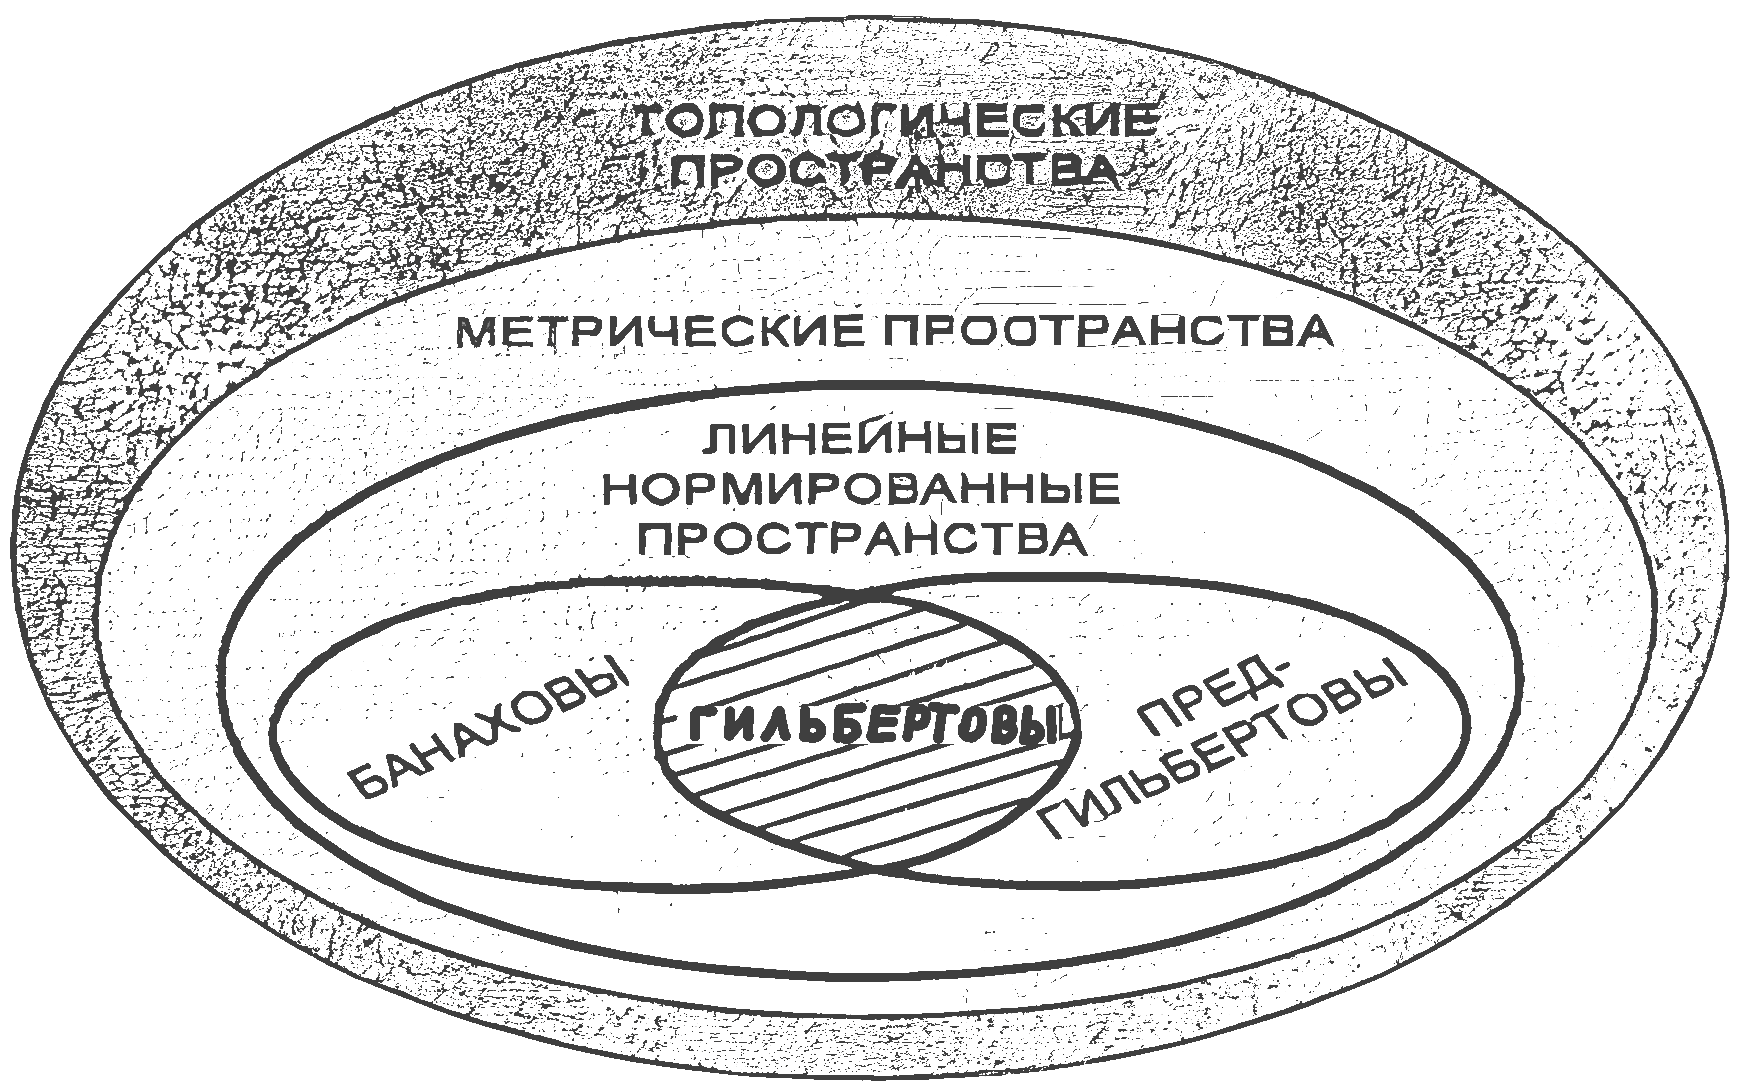
\includegraphics[width=0.5\textwidth]{/Users/vladbelousov/Desktop/Semestr_4-FP-NSU/ДфУ/Лекции_по_дням/image/1.png}
\end{center}

\begin{gather*}
   \text{З.С.Э: }  mgy_0+0= mgy(x)+ \frac{m |v| ^2}{2} \\
    \lvert v  \rvert =\sqrt{v_x ^2 + v_y ^2} = \sqrt{\left( \frac{\partial x}{\partial t}  \right) ^2 +\left( \frac{\partial y }{\partial t}  \right) ^2 }= \sqrt{1+(y'(x))^2} \frac{dx}{dt} \\
    \sqrt{2g(y_0- y(x)) }= |v|= \sqrt{1+(y(x)')^2} \frac{dx}{dt} \\
    T= \int_{0}^{T}dt= \int_{x_0 }^{x_1} \frac{\sqrt{1+(y'(x))^2}}{\sqrt{2g(y_0+ y(x)) }} dx   
\end{gather*}

\begin{flushleft}
    Пример 2 : задача поверхности вращения наименьшей площади. 
\end{flushleft}

\begin{center}
    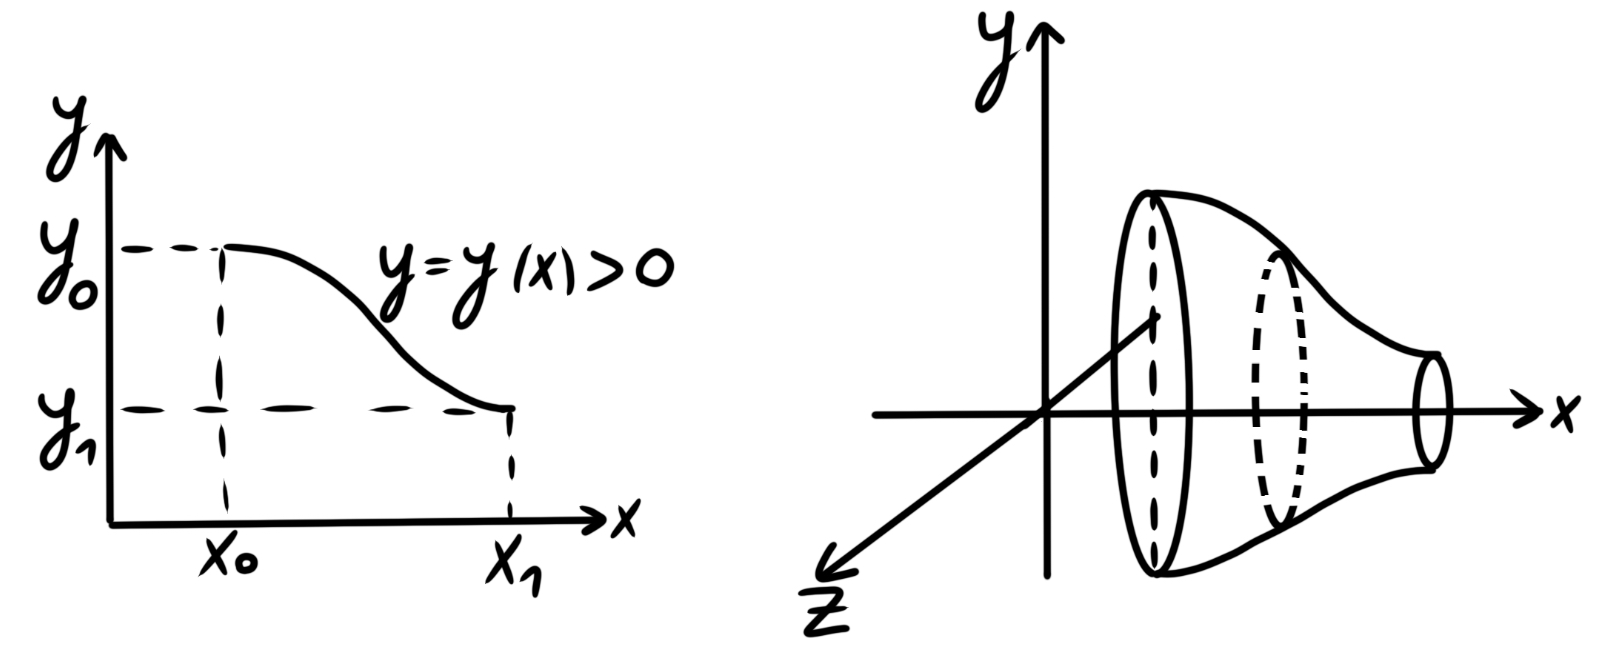
\includegraphics[width=0.8\textwidth]{/Users/vladbelousov/Desktop/Semestr_4-FP-NSU/ДфУ/Лекции_по_дням/image/2.png}
\end{center}

Площадь \( S \to \min  \) 

\begin{center}
    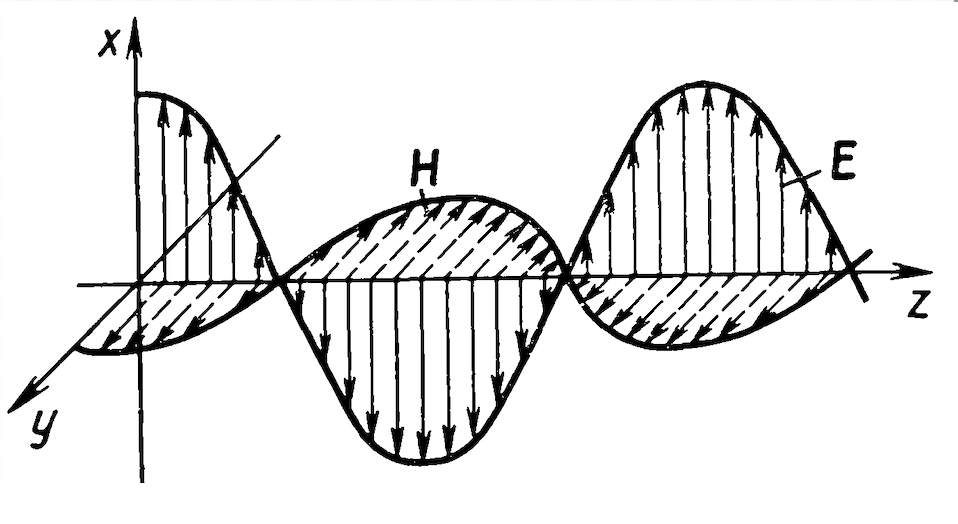
\includegraphics[width=0.5\textwidth]{/Users/vladbelousov/Desktop/Semestr_4-FP-NSU/ДфУ/Лекции_по_дням/image/3.png}
\end{center}

\begin{gather*}
    \Delta \delta= \sqrt{(\Delta x ) ^2 + ( \Delta y) ^2} = \sqrt{1 + \left( \frac{\Delta y}{\Delta x}  \right) ^2} \Delta x \\
    \Delta S = 2 \pi y (x) \Delta \delta \\
    \sum  \Delta S \xrightarrow{\Delta x \to  0}  \int_{x_1}^{x_2} 2 \pi y(x ) \sqrt{1+(y'(x))^2}dx  
\end{gather*}


\begin{flushleft}
    Пример 3 : задача о геодезических на поверхности.
\end{flushleft}

Найти кривую, проходящую через точки А и В, лежащую на поверхности, которая имеет наименьшую длину.

\begin{center}
    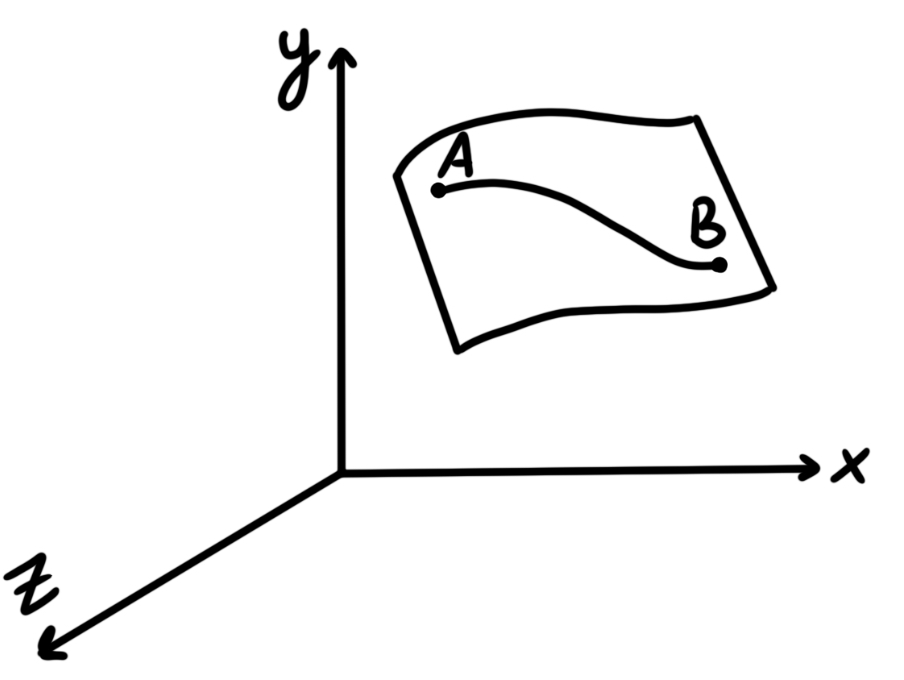
\includegraphics[width=0.4\textwidth]{/Users/vladbelousov/Desktop/Semestr_4-FP-NSU/ДфУ/Лекции_по_дням/image/4.png}
\end{center}
\begin{gather*}
    G(x,y,z)=0 - \text{уравнение поверхности} \\ 
    \text{Пусть уравнение кривой }:
    \begin{cases}
        x=x(t) \\
        y=y(t) \quad \quad t \in  [t_0,t_1] - \text{параметр} \\
        z= z(t)
    \end{cases}\\
    G(x(t),y(t),z(t)) = 0 \leftarrow \text{кривая лежит на поверхности}  \\
    l= \sum  \Delta l = \sum \sqrt{(\Delta x) ^2 + ( \Delta y ) ^2 + ( \Delta z ) ^2}=\sum  \sqrt{\left( \frac{\Delta x}{\Delta t} \right) ^2 + \left( \frac{\Delta y}{\Delta t} \right) ^2 + \left( \frac{\Delta z}{\Delta t} \right) ^2} \Delta t \\
    l \xrightarrow{\Delta t \to  0}    \int_{t_0}^{t_1} \sqrt{(x'(t)) ^2 + ( y'(t)) ^2 + ( z' ( t)) ^2 }dt  
\end{gather*}

\section{Простейшая задача вариационного исчисления}

\[ I[y]= \int_{x_0}^{x_1} F ( x, y(x),y'(x))dx \quad \quad \quad \quad (1)  \] 

\( F : \mathbb{D} \to \mathbb{R}, \mathbb{D} \subset \mathbb{R} ^3   \) непустое открытое множество, \( F \in  C ^2 (\mathbb{D}) \) 

\begin{definition}[допустимая функция]   
    Функция \( y : [x_0,x_1]\to \mathbb{R}  \) называется допустимой, если: 
    
    1) \(\displaystyle  y(x)\in  C([x_0,x_1]) \)
    
    2) \(\displaystyle  y(x) \in  C ^2 ((x_0,x_1)) \)
    
    3) \( \displaystyle \forall x \in  [x_0,x_1 ] , ( x, y(x), y ' (x)) \in  \mathbb{D}  \)
    
    4) \( \displaystyle \int_{x_0 }^{x_1} F(x,y(x),y' (x))dx \)  сходится

\end{definition}



\[ \text{Краевые условия: } y(x_0)=y_0,\text{ }  y(x_1)=y_1 \quad \quad \quad \quad (2) \] 

\begin{definition}
    Допустимая \( \tilde{y}:[x_0,x_1] \to  \mathbb{R}  \) доставляет локальный минимум функционалу (1) при краевых условиях (2),если: 

    1) \( \tilde{y}(x_0)=y_0, \tilde{y}(x_1)= y_1   \) 

    2) \( \exists \varepsilon_0 >0 \text{ }  \forall   \) допустимой функции \( y(x) \), удовлетворяющей (2): \( \sup _{x \in  [x_0,x_1]}|y(x)-\tilde{y}(x) |< \varepsilon_0  \) выполняется: \( I[\tilde{y}] \le I[y] \) 
\end{definition}

\begin{definition}
    Допустимая функция \( \tilde{y} : [x_0,x_1] \to  \mathbb{R} \)  доставляет глобальный минимум функционалу I[y] при краевых условиях (2), если: 

    1) \( \tilde{y} (x_0)=y_0, \text{ } \tilde{y} (x_1) =y_1 \)
    
    2) \( \forall \) допустимой функции \( y(x) \), удовлетворяющей (2), выполняется \( I[\tilde{y} ] \le I [y] \) 
\end{definition}

\section{Необходимые условия локального экстремума}

Аналог \( f'(x) = 0  \) 

Пусть функция \(\tilde{y}   \) доставляет функционалу \( I[y] \) при краевых условиях (2) локальный минимум \( \Rightarrow I[\tilde{y} ] \le I[y]  \), где \( y(x) \) из определенного локального минимума.

Возьмем \( \displaystyle y(x)=\tilde{y} + \varepsilon \eta(x) , \quad \varepsilon \in \left( -\frac{\varepsilon_0}{M}, \frac{\varepsilon_0}{M}   \right), \quad  M= \max _{x \in  [x_0,x_1]} |\eta (x) |  \)

\( \eta (x) \in  C ^2 ([x_0,x_1])  \) - финитная функция. 

\begin{minipage}{0.4\textwidth}
    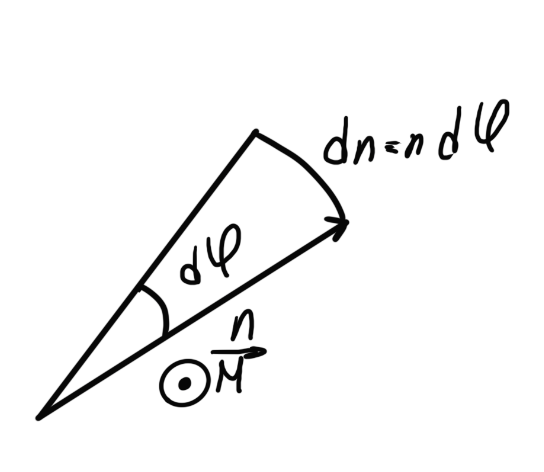
\includegraphics[width=\textwidth]{/Users/vladbelousov/Desktop/Semestr_4-FP-NSU/ДфУ/Лекции_по_дням/image/5.png}
\end{minipage}
\begin{minipage}{1\textwidth}
    \( \quad \quad \quad  \Rightarrow I[\tilde{y} ] \le I[\tilde{y} + \varepsilon \eta ]  \) 
\end{minipage}

Рассмотрим функцию \( g(\varepsilon)= I[\tilde{y}+ \varepsilon \eta  ] \Rightarrow g(0) \le g(\varepsilon) \) 

\begin{minipage}{0.25\textwidth}
    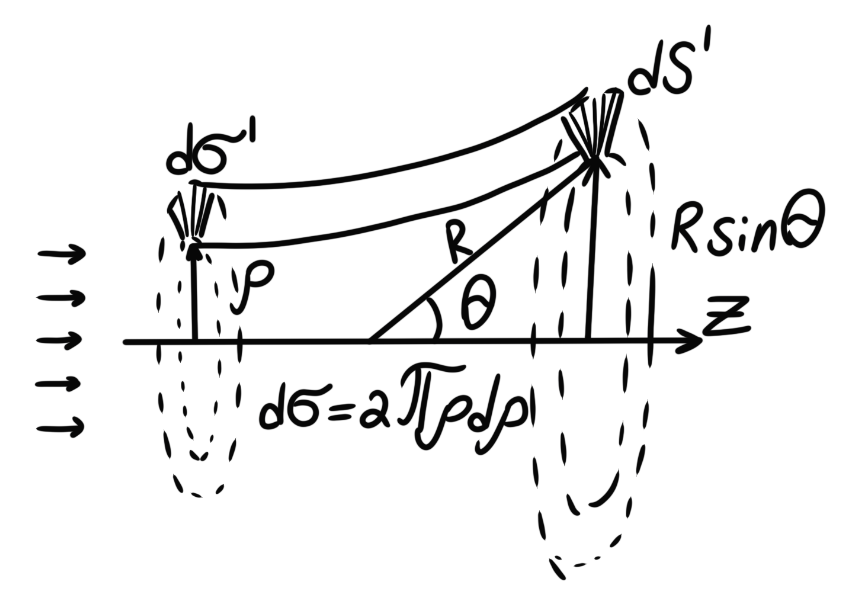
\includegraphics[width=\textwidth]{/Users/vladbelousov/Desktop/Semestr_4-FP-NSU/ДфУ/Лекции_по_дням/image/6.png}
\end{minipage}
\begin{minipage}{1\textwidth}
    \( \quad \varepsilon= 0 - \text{ точка локального минимума для функции } g(\varepsilon) \Rightarrow g'_{\varepsilon}(0)=0     \) 
\end{minipage}

\begin{gather*}
    0 = \frac{d}{d \varepsilon}g (\varepsilon) |_{\varepsilon=0}= \frac{d}{d \varepsilon} \left[ \int_{x_0}^{x_1} F(x,\tilde{y}+ \varepsilon\eta  (x) , \tilde{y}'+\varepsilon\eta ' (x) ) dx \right] \bigg |_{\varepsilon=0} \boxed{=}   \\
    \int_{x_0}^{x_1}= \underbrace{\int_{x_0}^{x_0+\delta} }_{(1)} +   \underbrace{\int_{x_0 +\delta}^{x_1-\delta} }_{(2)}  +\underbrace{\int_{x_1 -\delta}^{x_1} }_{(3)} \quad ; \quad \frac{d}{d \varepsilon} I_1= \frac{d}{d \varepsilon} I_2=0 \\   
\end{gather*}
\begin{theorem}[из математического анализа]
    \( f(x, \varepsilon): [a,b] \times [c,d] \to \mathbb{R}  \) - непрерывна, \( \displaystyle \exists  \frac{df}{d \varepsilon} (x, \varepsilon)   \)  - непрерывна
    \[ \Rightarrow \frac{d}{d \varepsilon} \int_{a}^{b} f(x, \varepsilon)dx= \int_{a }^{b } \frac{d}{d \varepsilon } f(x, \varepsilon)dx     \]  
\end{theorem}  

Вносим производную под знак интеграла: 

\begin{gather*}
    \boxed{=} \int_{x_0 + \delta}^{x_1- \delta}\left[ \frac{\partial F}{\partial y }(\dots) \eta (x )+ \frac{\partial F}{\partial y'} \eta '(x)   \right] dx \bigg |_{\varepsilon=0}=   \int_{x_0 + \delta}^{x_1- \delta}\frac{\partial F}{\partial y }(\dots) \eta (x )dx+ \underbrace{\frac{\partial F}{\partial y'}(x) \eta (x) \bigg |^{x_1- \delta}_{x_0+\delta}    }_{=0}- \\
    -\int_{x_0 + \delta}^{x_1- \delta} \eta (x )\frac{d}{dx } \left[ \frac{\partial F}{\partial y' }(\dots) \right] dx \bigg | _{\varepsilon=0} =\int_{x_0 + \delta}^{x_1- \delta} \left[ \frac{\partial F}{\partial y}(\dots)- \frac{\partial}{\partial x} \frac{\partial F}{\partial y'}(\dots)    \right]\eta(x) dx \bigg |_{\varepsilon=0}  \boxed{=}  \\
    \boxed{=} \int_{x_0 }^{x_1} \eta(x) \left[ \frac{\partial F}{\partial y}(x,y(x),y'(x)) -  \dots \right] dx =0
\end{gather*}

\( \forall   \) финитной функции \( \eta (x)  \)

\begin{lemma}[основаная леммая вариационного исчисления]
    \( f(x) : [x_0,x_1] \to  \mathbb{R} -\) непрерывна и  \( \displaystyle \int_{x_0}^{x_1} f(x)\eta (x)dx=0, \forall   \) финитной \( \eta (x) \). Тогда \( f(x) \equiv 0 \text{ } \forall x \in  [x_0,x_1]   \) 
\end{lemma}

По лемме: \( \displaystyle \frac{\partial F}{\partial y}- \frac{d}{dx} \frac{\partial F}{\partial y '} =0     \) - необходимое условие локального экстремума( \textbf{уравнение Эйлера} )

\begin{definition}[экстремаль]
    Допустимая функция \( y(x) \) называется экстремалью функционала \( I[y] \)  при краевых условиях (2), если: 

    1) \( y(x_0)=y_0, \text{ } y(x_1)=y_1  \) 

    2) \( y(x) \) удовлетворяет условию Эйлера
\end{definition}


%%-------------------------------%%

% Закрытие документа, если файл компилируется отдельно
\ifdefined\mainfile
    % Если это основной файл, не нужно заканчивать документ
\else
    \end{document}
\fi
% Условная компиляция для самостоятельной работы
\ifdefined\mainfile
    % Если это часть основного файла, не добавляем начало и конец документа
\else
    \documentclass[12pt, a4paper]{report}
    \usepackage{/Users/vladbelousov/Desktop/Semestr_4-FP-NSU/Настройка/library}
    \usepackage[utf8]{inputenc} % Подключение поддержки UTF-8
    \begin{document}
\fi

%%-------------------------------%%

\[ \begin{aligned}
\begin{cases}
    \displaystyle I[y] = \int_{x_0}^{x_1} F(x,y(x),y'(x))dx \\
    y(x_0)=y_0, \text{ } y(x_1)=y_1
\end{cases}
\quad (1)
\end{aligned} \] 

Найти функцию \( y(x) \)   такую, чтобы функционал \( I[y] \) принимал наибольшее или наименьшее значение. 

Необходимо найти условие локального экстремума: 

Если \( \tilde{y }       \)  экстремум \( \Rightarrow \tilde{y }  \frac{\partial F }{\partial y} - \frac{d}{dx }  \frac{\partial F}{\partial y '} = 0 \quad (2)   \)

\begin{proof}[Докозательство формулы (2)]
    \[ I[\tilde{y}] \le I[y] , y = \tilde{y} + \varepsilon \eta , \varepsilon \in  (- \varepsilon_1, \varepsilon_1), \eta(x) \in C^2([x_0,x_1])  - \text{финитная }    \] 
    
    \begin{center}
        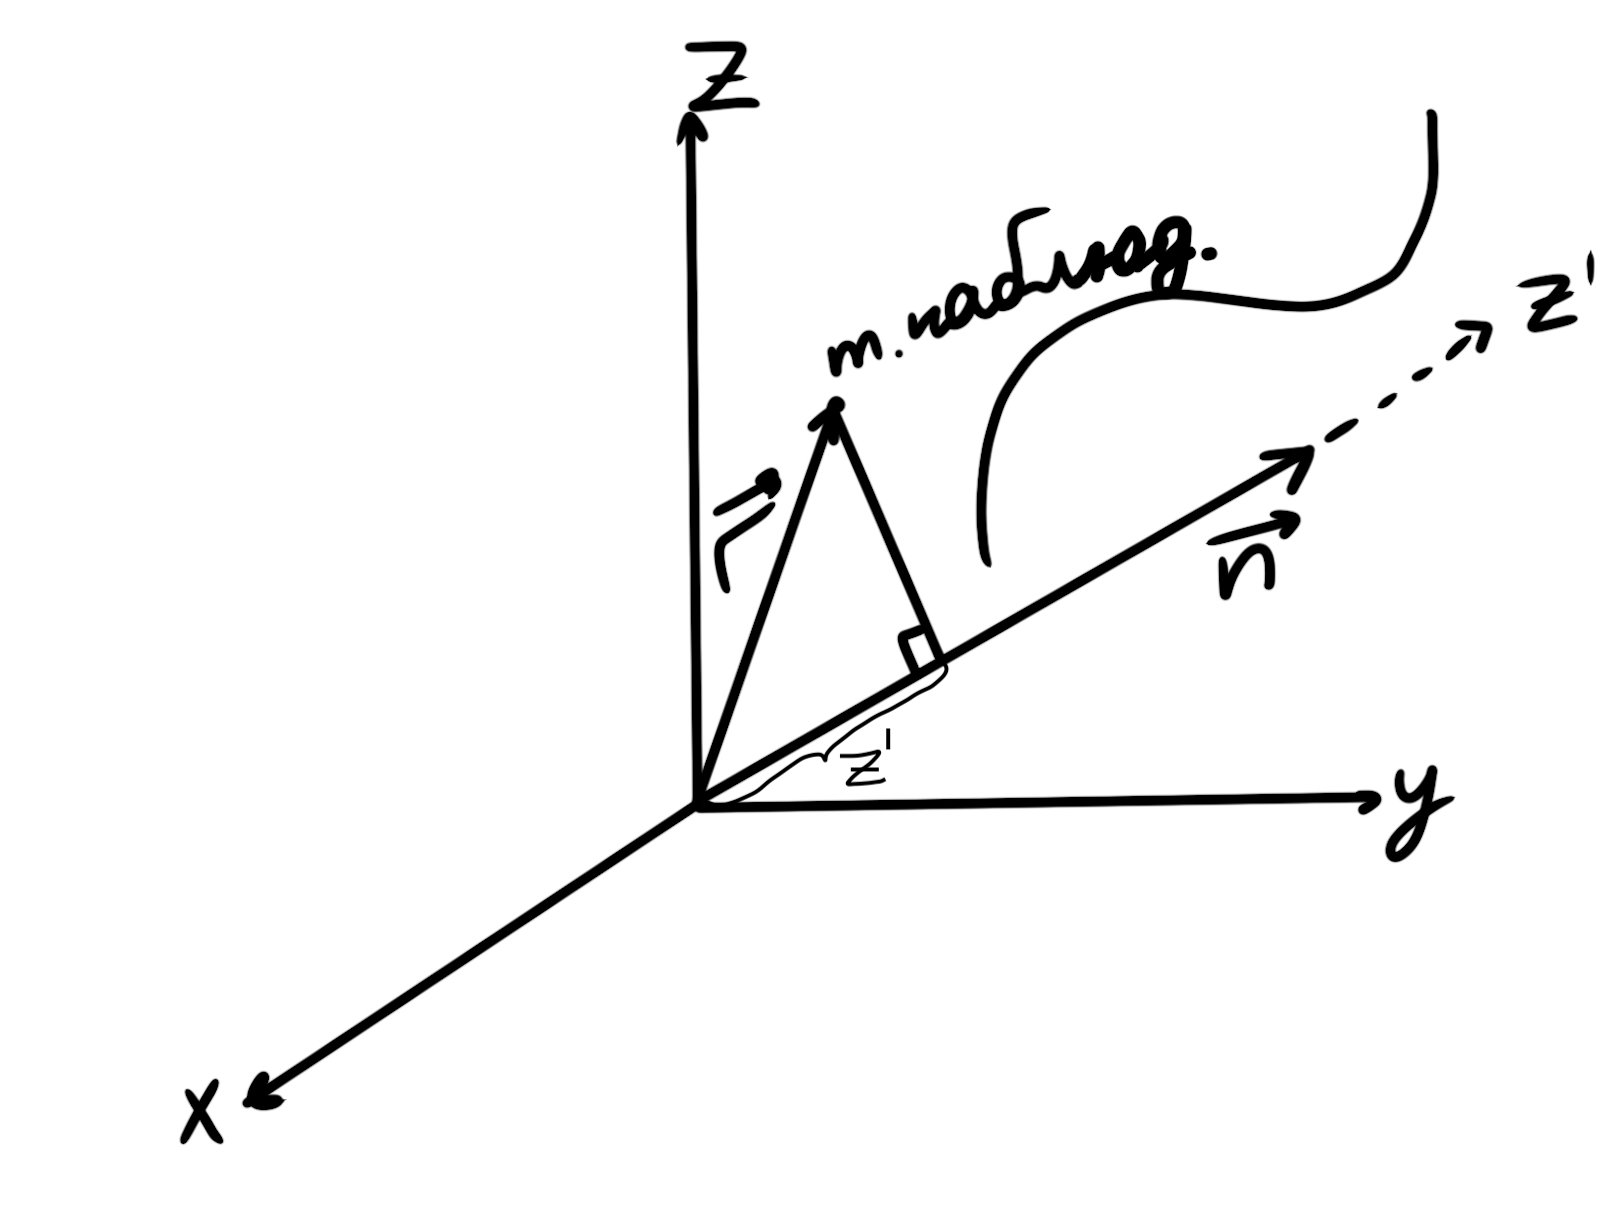
\includegraphics[width=0.3\textwidth]{/Users/vladbelousov/Desktop/Semestr_4-FP-NSU/ДфУ/Лекции_по_дням/image/7.png}
    \end{center}

    \[ \underbrace{I[y]}_{= g(0)} \le \underbrace{I[\tilde{y}+ \varepsilon \eta ]}_{=g(\varepsilon)} \Rightarrow g(0) \le g(\varepsilon) \Rightarrow g'( 0) = 0\] 

    \[ 0= \frac{d}{d \varepsilon} g(\varepsilon) |_{\varepsilon= 0 }= \int_{x_0}^{x_1} \left( \frac{\partial F }{\partial y } ( x , \tilde{y}(x) , \tilde{y }' (x) ) - \frac{d}{dx }  \frac{\partial F }{\partial y' } ( x , \tilde{y}(x) , \tilde{y }' (x) )  \right) \eta (x) dx , \forall \eta (x)  - \text{финитная}    \] 

    \begin{lemma}[Лагранжа]     
        Пусть \( f(x) \) - непрерывна и \( \displaystyle \int_{x_0}^{x_1} f(x) \eta (x) dx =0. \forall \eta (x) \) - финитная на \( [x_0,x_1] \). Тогда \( f(x) = 0 , \forall x \in  [x_0,x_1] \) 
    \end{lemma}

    \begin{proof}
        От противного:
        \begin{center}
            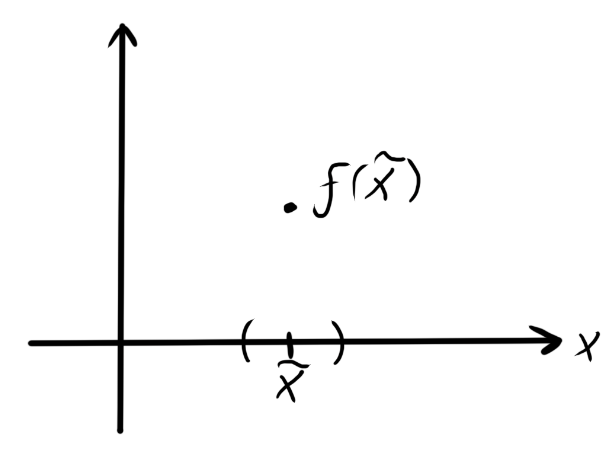
\includegraphics[width=0.3\textwidth]{/Users/vladbelousov/Desktop/Semestr_4-FP-NSU/ДфУ/Лекции_по_дням/image/8.png}
        \end{center}
        Пусть для определенности \( f(\tilde{x } )> 0        \) . Тогда так как \( f(\tilde{x}) \) - непрерывна, то \( f(x)>0    \) при \( x \in (\tilde{x}- \delta_0, \tilde{x}+\delta_0) \) 

        Возьмем функцию \( \eta(x) = \begin{aligned}
            \begin{cases}
                (\delta_0 ^2 - (x- \tilde{x})) ^ 4 , |x- \tilde{x}|< \delta   \\
                0 , |x- \tilde{ x } | > \delta_0
                \end{cases}
                - \text{финитная функция} 
        \end{aligned}\)
        
        \begin{center}
            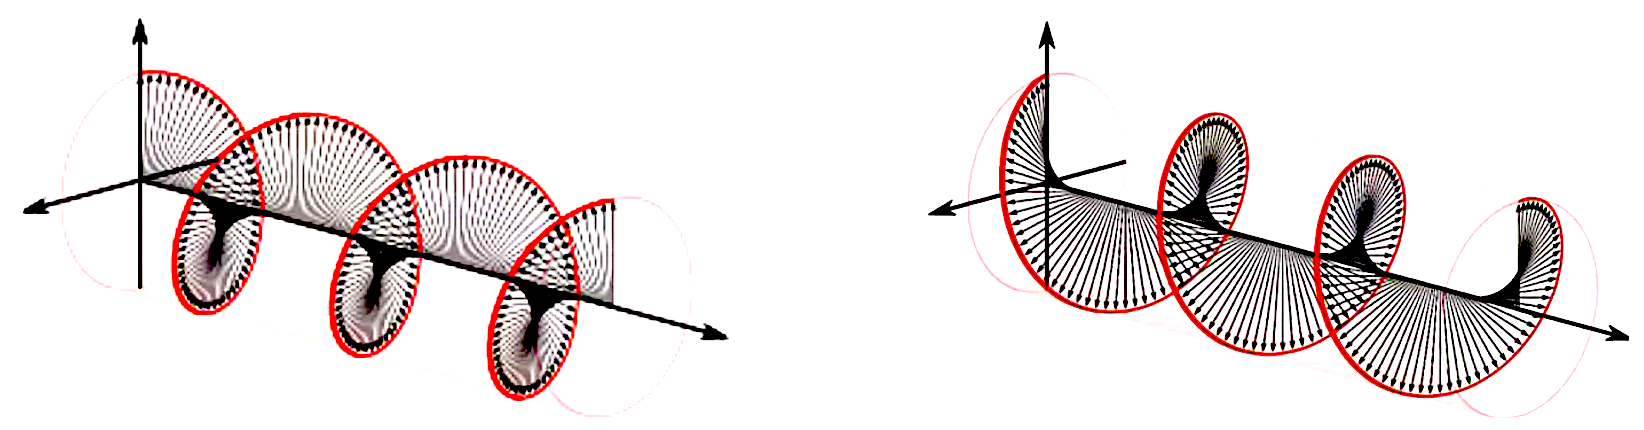
\includegraphics[width=0.3\textwidth]{/Users/vladbelousov/Desktop/Semestr_4-FP-NSU/ДфУ/Лекции_по_дням/image/9.png}
        \end{center}

        \[ \int_{ x_0 }^{x_1} f(x ) \eta(x ) dx = \int_{x_0 - \delta_0}^{x_1- \delta_0} \underbrace{f(x)}_{>0} \underbrace{\eta( x)}_{>0} dx >0 - \text{противоречие}    \] 

        \[ \Rightarrow \forall x \in  [x_0, x_1] : f(x) = 0  \] 
    \end{proof}

    Из доказательства леммы следует, что доказана формула (2)
\end{proof}

\section{Случай понижения порядка в уравнении Эйлера}   

\[ \frac{\partial F}{\partial y} - \frac{d}{d x }  \frac{\partial F}{\partial y'} = 0 \quad  F=F(x,y(x),y'(x))  \] 

1) \(\displaystyle  F= f(x,y) \Rightarrow \frac{\partial F }{\partial y} (x,y) =0 \Rightarrow y= y(x)    \) 

2) \( \displaystyle F= F (x, y ') \Rightarrow \frac{d}{dx }  \frac{\partial F }{\partial y'} (x,y') =0 \Rightarrow \frac{\partial F }{\partial y'} (x,y') = C    \) 


3) \( F= F( y , y ') \) :

\[ \frac{\partial F }{\partial y } - \frac{d}{dx }  \frac{\partial F }{\partial y '} = 0 | \cdot y '     \] 

\[ y' \frac{\partial F }{\partial y } - \underbrace{y ' \frac{ \partial F }{\partial y '}}_{= \frac{d}{dx } \left( y ' \frac{\partial F }{\partial y '} \right)- y'' \frac{\partial F }{\partial y '} }    = 0 \] 

\[ y' \frac{\partial F }{\partial y } - \frac{d}{dx } \left( y ' \frac{\partial F }{\partial y '}  \right)+ y'' \frac{\partial F }{\partial y '}  = 0 \] 

Заметим, что: \( \displaystyle \frac{d}{dx }F(y,y')  = y' \frac{\partial F }{\partial y } + y '' \frac{\partial F }{\partial y '}   \) 

\[ \frac{d}{dx }  F - \frac{d}{dx } \left( y ' \frac{\partial F }{\partial y '}           \right) = 0 \Rightarrow \boxed{F- y ' \frac{\partial F }{\partial y '} = C}   \] 


\section{Решение задачи о брахистохроне}

\begin{center}
    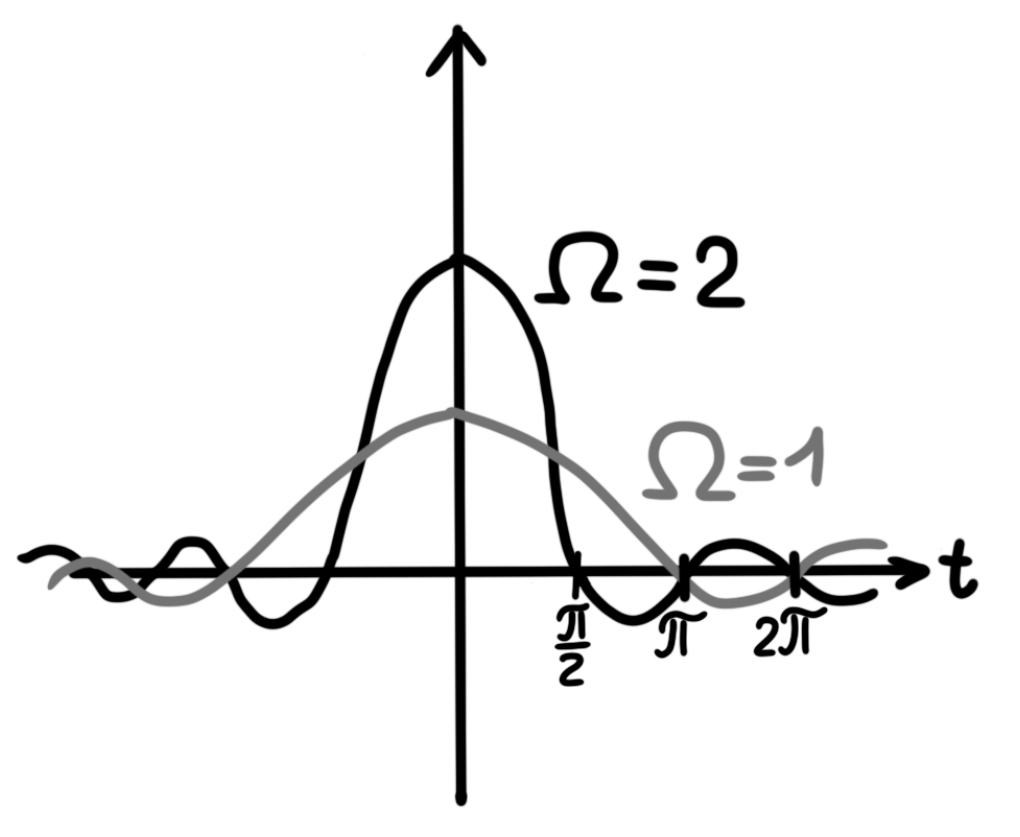
\includegraphics[width=0.3\textwidth]{/Users/vladbelousov/Desktop/Semestr_4-FP-NSU/ДфУ/Лекции_по_дням/image/10.png}
\end{center}

\[ \begin{cases}
\displaystyle I[y] = \int_{x_0}^{x_1} \frac{\sqrt{ 1+ (y ' (x)) ^2 )}}{\sqrt{2 g (y_0 - y (x))}} dx \\
y(x_0) = y_0, \text{ } y(x_1) = y_1
\end{cases} \] 

\[ \frac{\sqrt{1+ ( y ' ) ^2 } }{ \sqrt{2 g ( y_0 - y )} } - y ' \frac{1}{\sqrt{1+ ( y ' ) ^2 }} \frac{2 y '}{2 \sqrt{1 +( y ') ^2 } } = C    \] 

\[ \underbrace{\sqrt{1+ ( y ' ) ^2 } - (y ') ^2 \frac{1}{ \sqrt{1 + (y') ^2}}}_{\displaystyle \frac{1}{\sqrt{1+ (y ') ^2 }} } = C \sqrt{2g (y_0 - y )}  \] 

\[ 1= \underbrace{c ^2 2g}_{= \frac{1}{c_1}>0 } ( y_0 - y)( 1+ (y ') ^2) \] 

\[ c_1= (y_0 - y )(1 + ( y ' ) ^2 ) \Rightarrow \pm \sqrt{\frac{c_1}{y_0 - y }-1} = y ' \quad (3 )  \] 

\begin{center}
    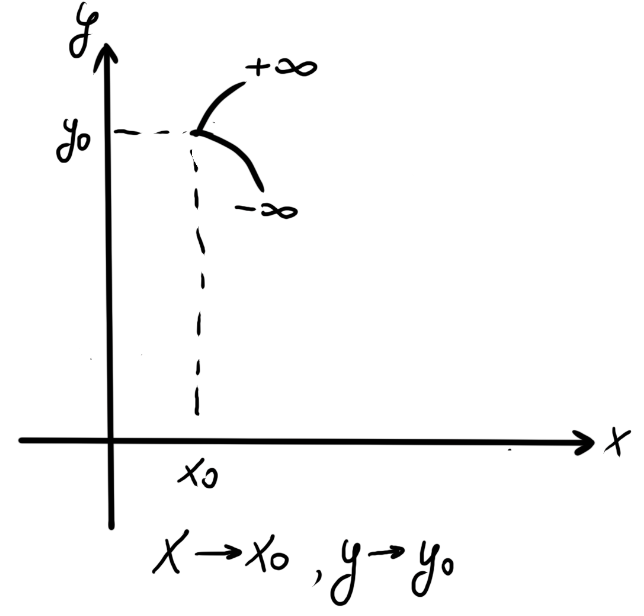
\includegraphics[width=0.3\textwidth]{/Users/vladbelousov/Desktop/Semestr_4-FP-NSU/ДфУ/Лекции_по_дням/image/11.png}
\end{center}

\[ 1+(y'(x)) ^2 = \frac{c_1}{y_0 - y(x)} \xrightarrow{x \to x_1} + \infty     \] 

\[ y ' ( x ) \xrightarrow{x \to  x_0} \underset{{\small \text{выбор}} : - }{\pm \infty}  \Rightarrow y ' (x )  \xrightarrow{x \to  x_0} - \infty      \] 

\[ y ' = - \sqrt{\frac{c_1- y_0 + y }{y_0 - y } } \] 

Замена: \( \tilde{y }= y_0 - y (x) \):

\[ \tilde{y} '(x) = + \sqrt{\frac{c_1 - \tilde{y }}{\tilde{y }} }  \] 

Замена: \( \tilde{y } = c_1 z \): 

\[ c_1 z ' = \sqrt{\frac{c_1 - c_1 z }{c_1 z } }= \sqrt{\frac{1-z}{z } } \] 

Замена: \( z= \sin ^2 s, s \in  \left[ 0 , \frac{\pi}{2}  \right] \) 

\[ c_1 2 \sin s \cos s \cdot s' = \sqrt{ \frac{1- \sin ^2 s }{\sin ^2 s } }= \frac{\cos s }{\sin s } \text{ } (\text{знак определили из интервала s} )   \] 

\[ 2 c_1 \sin ^2 s \frac{ds}{dt } =1     \] 

\[ \frac{dx }{ds }  = c_1 ( 1 - \cos (2s) ) \Rightarrow \boxed{x(s) = c_1 \left( s - \frac{1}{2 }  \sin 2s  \right)- c_2} -   \] 

\[ y(x )= y_0 - \tilde{y } (x ) = y_0 - c_1z= y_0 - c_1 \sin ^2 s = y_0 - \frac{c_1}{2} ( 1 - \cos  2s) \]  

\[ \boxed{y(s )= y_0 - \frac{c_1}{2 }  ( 1 - \cos (2s))}   \] 

Замена: \( t = 2s , \text{}  t \in  ( 0 , \pi) \) 

\[ \begin{aligned}
    \begin{cases}
        \displaystyle x(t) = \frac{c_1}{ 2 }  ( t - \sin t ) + c_2  \\ 
        \displaystyle y(t)= y_0 - \frac{c_1}{2 }  ( 1 - \cos t)
    \end{cases}
    \quad , \quad t \in ( 0 , \pi)
\end{aligned} \]

\[ \begin{pmatrix}
x(t )\\
y (t)
\end{pmatrix} = \begin{pmatrix}
\frac{c_1}{2 }  + c_2 \\
y - \frac{c_1}{2} 
\end{pmatrix}= \begin{pmatrix}
-\frac{c_1}{2 } \sin t\\
\frac{c_1}{2}  \cos t 
\end{pmatrix} \quad t \in  (0 , \pi)\] 

\begin{center}
    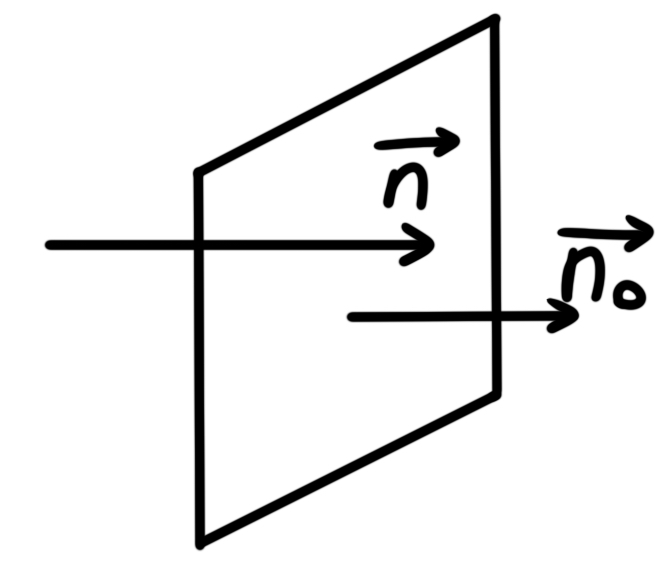
\includegraphics[width=0.5\textwidth]{/Users/vladbelousov/Desktop/Semestr_4-FP-NSU/ДфУ/Лекции_по_дням/image/12.png}
\end{center}

\[ \begin{aligned}
    t= 0 : 
    \begin{cases}
        x(0 ) = c_2 = x_0 \\
        y(0 ) = y_0
    \end{cases}
\end{aligned} \] 

\[ \begin{aligned}
    t= \pi: 
    \begin{cases}
        x(\pi ) = \frac{c_1}{2 }  \pi + c_2= \frac{c_1}{2 } \pi + x_0  \\
        y(\pi) = y_0 - c_1
    \end{cases}
\end{aligned} \] 

\begin{center}
    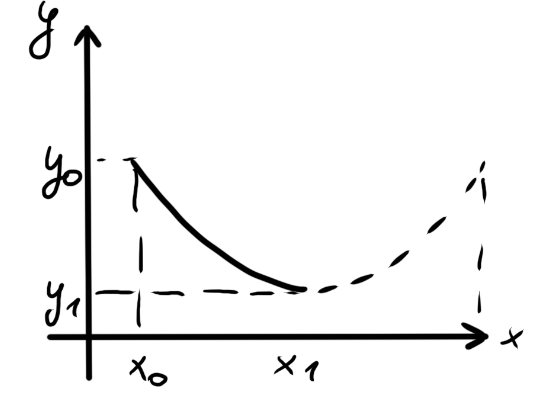
\includegraphics[width=0.3\textwidth]{/Users/vladbelousov/Desktop/Semestr_4-FP-NSU/ДфУ/Лекции_по_дням/image/13.png}
\end{center}

Теперь возьмем "+" ( формула (3)): 

\[ y ' = \sqrt{\frac{ c_1 - y_0 + y }{y_0 - y } }\quad (5 ) \] 

\[ \tilde{y } (x ) = y_0 - y (x ) \Rightarrow \tilde{y } ' = - \sqrt{\frac{ c- \tilde{ y } }{\tilde{y }}}   \]  

Делаем те же действия (замены) и получаем такие же \( x(s), y ( s ) \) с различием только в интервале для t: 

\[ \begin{aligned}
    \begin{cases}
        x(T)  = \frac{C_1}{ 2 }  ( t- \sin t ) + x_0 \\
        y(t ) = y_0 - \frac{c_1}{2 }  ( 1- \cos  t )            
    \end{cases}
    \quad ,\quad t \in ( 0 , 2 \pi ) \Rightarrow \text{ циклоида полная }  
\end{aligned} \]  

\begin{center}
    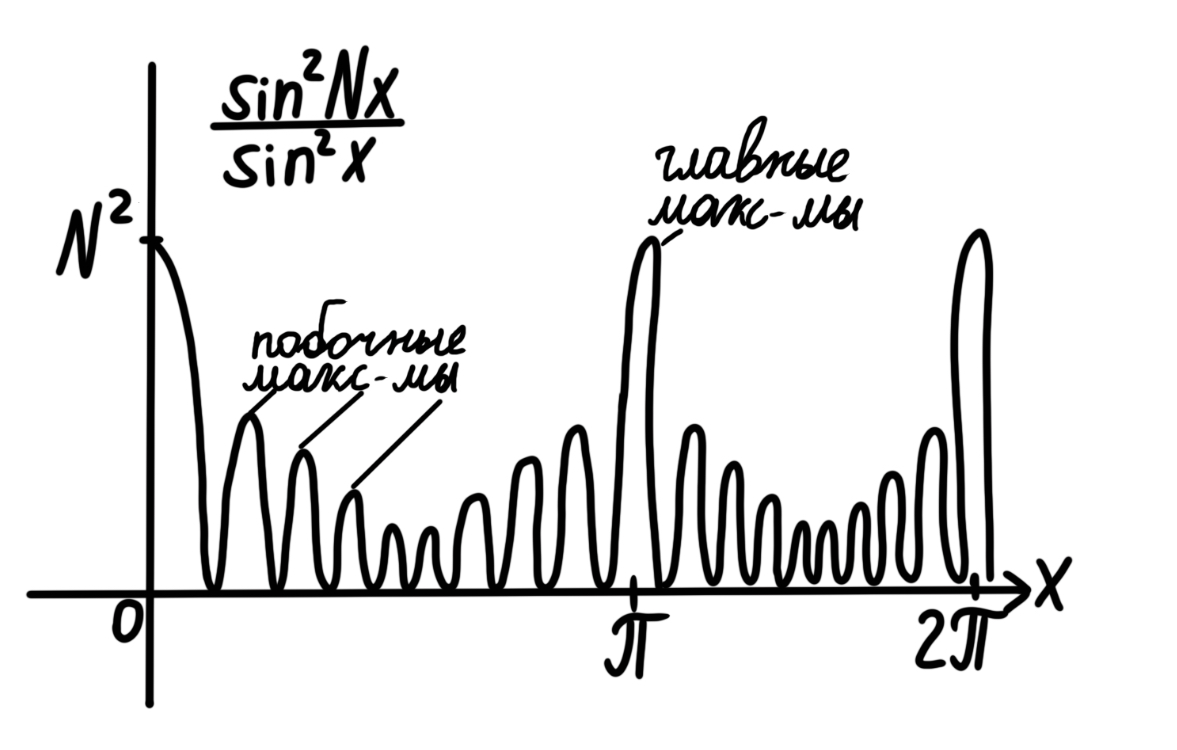
\includegraphics[width=0.5\textwidth]{/Users/vladbelousov/Desktop/Semestr_4-FP-NSU/ДфУ/Лекции_по_дням/image/14.png}
\end{center}

\newpage

\section{ Решение задачи о поверхности вращения наименьшей площади}

\begin{center}
    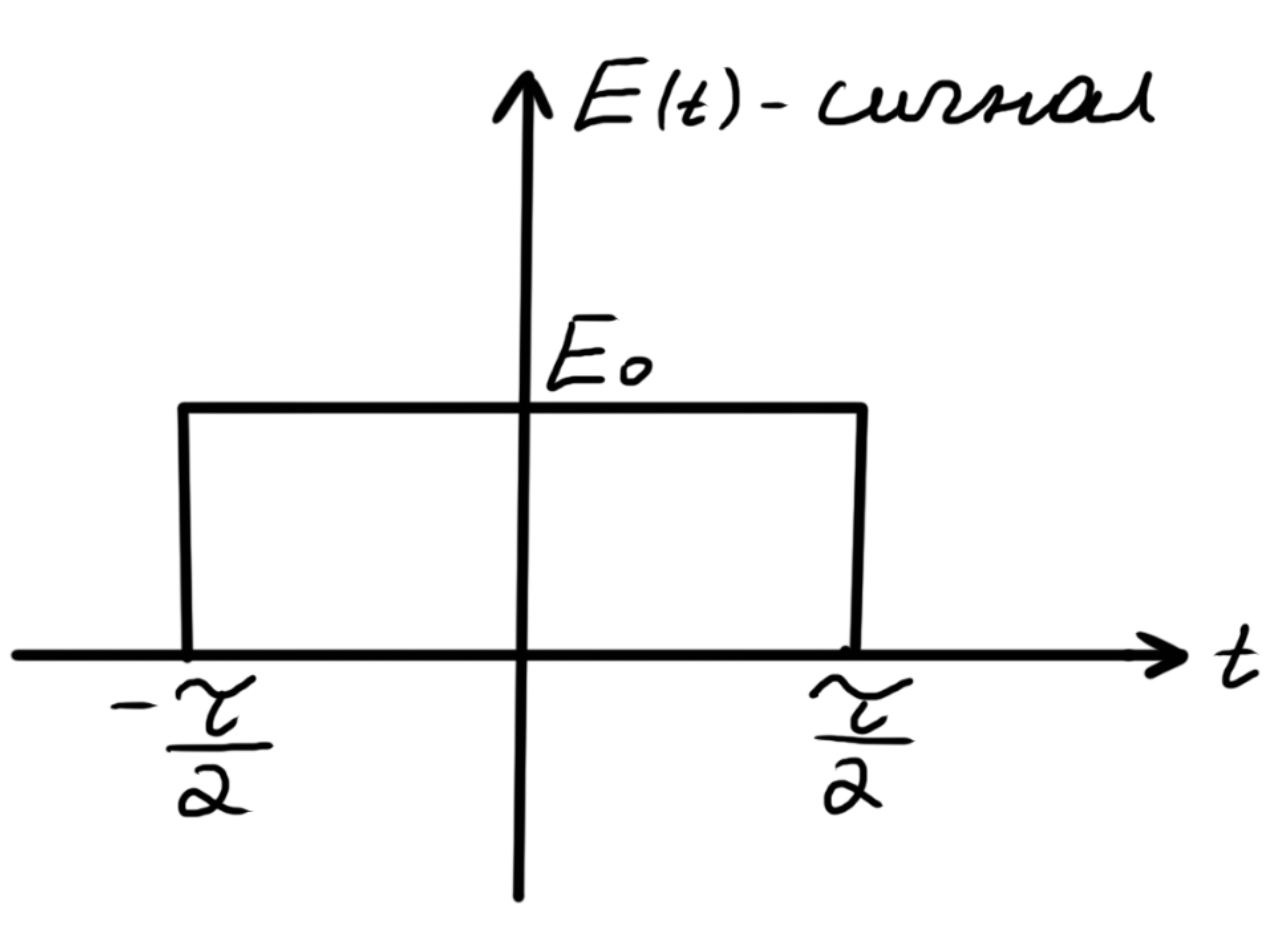
\includegraphics[width=0.3\textwidth]{/Users/vladbelousov/Desktop/Semestr_4-FP-NSU/ДфУ/Лекции_по_дням/image/15.png}
\end{center}

\[ \begin{cases}
I[ y ] = \int_{x_0}^{x_1} 2 \pi y(x )  \sqrt{1 + (y '(x ) ^2 )} \\ 
y( x_0 ) = y_0 , \text{ }  y ( x_1 ) = y_1 
\end{cases} \] 

\[ F- y; \frac{\partial  F }{\partial   y' } = C   \] 

\[ 2 \pi y \sqrt{ 1 + (y' ) ^2 } - y ' 2 \pi y \frac{2 y '}{ 2 \sqrt{1 + ( y ') ^2 }} = C  \] 

\[ 2 \pi y \underbrace{\left( \sqrt{1 + (  y') ^2 } - \frac{ (y ' ) ^2 }{\sqrt{1 + ( y ' ) ^2 }}  \right)}_{= \frac{1}{\sqrt{ 1 + ( y ' ) ^2 }} } = C \] 

\[ ( 2 \pi y  ) ^2 = c ^2 ( 1 + ( y '   ) ^2 ) \] 

1) \( c= 0 \Rightarrow y(x )  =0  \) - решение, если \( y_0 = y_1 = 0 \) 

2) \( c \neq 0 \Rightarrow \left(  \frac{y}{c_1 }     \right) ^2 = 1 + ( y ' ) ^2 \Rightarrow y ' = \pm  \sqrt{\frac{ y ^2 }{c_1 ^2} - 1  }, \text{ }  c_1 = \frac{c}{2 \pi} > 0         \) 

\[ y( x ) = \mathrm{ch}  z(x  ) c_1 , \text{ }  z> 0 \]  

\[ c_1 \mathrm{sh } z \cdot z ' (x )   =\pm \underbrace{ \sqrt{\mathrm{ch} ^2 z - 1  }}_{= \mathrm{sh} z  }   \Rightarrow c_1 z = \pm 1   \] 

\[ z= \pm  \frac{ x- c_2 }{c_1} \Rightarrow y ( x )  = c_1 \mathrm{ch} \left( \frac{x+c_2 }{c_1}  \right)  - \text{цепная линия}  \] 

\begin{center}
    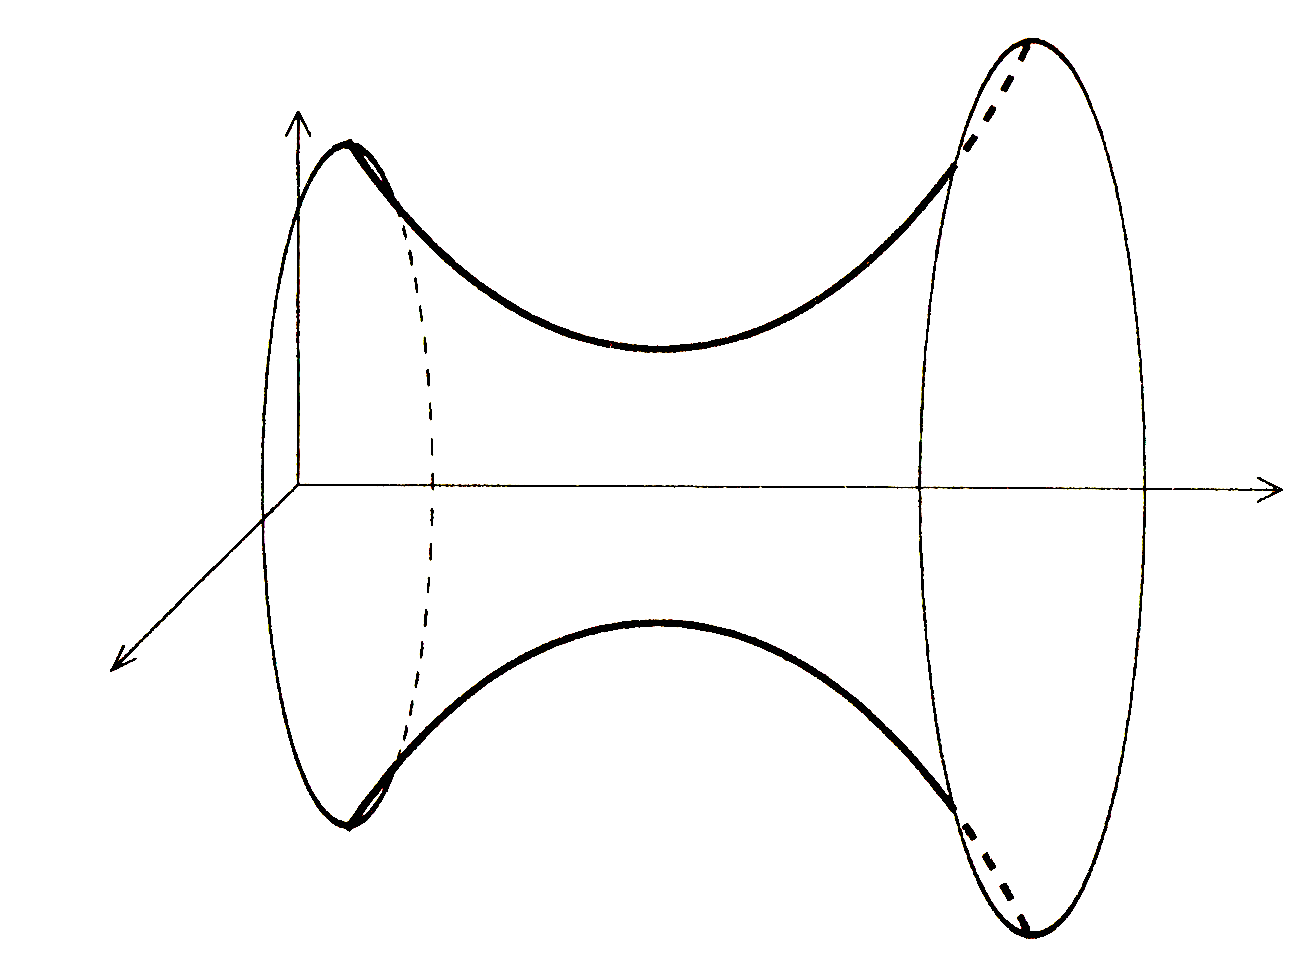
\includegraphics[width=0.4\textwidth]{/Users/vladbelousov/Desktop/Semestr_4-FP-NSU/ДфУ/Лекции_по_дням/image/16.png}
\end{center}



\section{Вариационная задача с несколькими функциями}

\[ I[y_1, \ldots, y_n ] = \int_{x_0 }^{x_1 } F(x,y_1(x),y_1 ' (x), \ldots , y_n ( x ) , y _n '( x))dx  \] 

\[ \begin{cases}
    y_1(x_0 ) = y_{01} , \ldots , y_n ( x_0 ) = y_{0n } \\
    y_1(x_1 ) = y_{11} , \ldots , y_n ( x_1) = y_{1n }
\end{cases} \] 

Необходимое условие локального экстремума: 

Пусть \( \tilde{y }_1 (x ) ,\ldots, \tilde{y }_n( x )  доставляет функционалу локальному экстремуму ему, то есть: \)

\[ I [\tilde{y }_1, \ldots , \tilde{y}_n  ] \le I[y_1, \ldots , y_n ] , \text{ }  \forall y_2, \ldots , y_n \] 

Можно взять \( y_1   \) - любое: \( y_2=\tilde{y}_2, \ldots ,   \) 

\[\Rightarrow \underbrace{ I[\tilde{y}_1, \ldots, \tilde{y   }_n ]}_{Y[\tilde{y } _1] } \le \underbrace{I[y_1, \ldots, \tilde{y  }_n ]}_{Y[y_1 ]} \Rightarrow \frac{\partial F }{\partial  y_1} - \frac{d}{dx }  \frac{\partial  F }{\partial  y_1 '}= 0     \]  

Аналогично: \( \frac{\partial F }{\partial  y_j }- \frac{d}{dx }  \frac{\partial F }{\partial  y ' _j} = 0   \) 


%%-------------------------------%%

% Закрытие документа, если файл компилируется отдельно
\ifdefined\mainfile
    % Если это основной файл, не нужно заканчивать документ
\else
    \end{document}
\fi
% Условная компиляция для самостоятельной работы
\ifdefined\mainfile
    % Если это часть основного файла, не добавляем начало и конец документа
\else
    \documentclass[12pt, a4paper]{report}
    \usepackage{/Users/vladbelousov/Desktop/Semestr_4-FP-NSU/Настройка/library}
    \usepackage[utf8]{inputenc} % Подключение поддержки UTF-8
    \begin{document}
\fi

%%-------------------------------%%

\section{ Вариационная задача с высшими производными }

\[ I[y ]= \int_{x_0 }^{x_1 } F( x, y (x), y' (x),..., y ^{(n )} (x))  dx\]  

\[ \begin{cases}
    y(x_0) = y_0 ,\quad  y (x_1) = y_1 \\
    y ' (x_0) = y ' _0 , \quad y ' (x_1) = y ' _1 \\
    \ldots 
    y^{(n )} = y^{(n )}_0, \quad y^{(n )} (x_1) = y^{(n )}_1
\end{cases} \]  

Необходимое условие локального экстремума: 

Если функция \( \tilde{y }(x ) \)  доставляет функционалу локальному экстремум, то \( \tilde{ y }(x) \)  - решение диффернциального уравнения

\[ \frac{\partial  F }{\partial  y } - \frac{d}{dx } \frac{ \partial  F }{\partial  y ' } + \frac{d ^2 }{dx ^2 } \frac{\partial  F }{\partial  y ''} + \ldots + \frac{d ^n }{dx ^n } \frac{\partial  F }{\partial  y ^{(n )}} = 0    \] 


\begin{proof}
     \[   \] 
    Пусть \( \tilde{y }( x) \)  доставляет функционалу локальный минимум \( \Rightarrow  \exists \varepsilon_0 >0 , \text{ }  \forall  y(x )\), удовлетворяет краевым условиям, \( \displaystyle \sup_{x \in [x_0 , x_1 ] } |y(x)-\tilde{y }(x) | < \varepsilon_0  \Rightarrow I[\tilde{y }] \le  I[y] \) 

    Возьмем \( y(x ) = \tilde{y }( x ) + \varepsilon \eta ( x ), \eta(x) \)  финитная функция.

    \[ \underbrace{I[\tilde{ y }]}_{g(0)} \le  \underbrace{I[\tilde{y }+ \varepsilon \eta ]}_{g(\varepsilon)} \Rightarrow g(0 ) \le  g(\varepsilon) \Rightarrow \varepsilon = 0  - \text{ точка локального минимума для функции } g(\varepsilon) \] 

    \[ g ' (0 ) = 0 \]  

    \[ 0 = \frac{d}{d \varepsilon } g(\varepsilon ) \bigg |_{\varepsilon = 0 }  = \frac{d}{d \varepsilon} \int_{x_0 }^{x_1} F ( x, \tilde{y }( x)  + \varepsilon \eta ( x ), \tilde{y }' ( x) + \varepsilon \eta' ( x ), ...) dx \bigg |_{\varepsilon = 0} \] 

    Если \( F \in C^{\infty  } (\mathbb{R} ^{n +2 } ), y(x ) \in C^{\infty  } ([x_0 , x_1 ])    \), то 

    \[ 0 = \int_{x_0 }^{x_1} \left[ \frac{\partial  F }{\partial  y } \eta( x) + \frac{\partial F }{\partial  y' }(... )\eta' ( x )+ \frac{\partial F }{\partial y ''} (...) \eta''(x) +\dots  \right]  dx \bigg | _{\varepsilon = 0 }  =    \] 

    \[ =\int_{x_0 }^{x_1}  \frac{\partial  F }{\partial  y } \eta ( x ) dx + \frac{\partial  F } {\partial  y ' } \eta  ( x ) \bigg |_{x_0 }^{x_1}   - \int_{x_0 }^{x_1} \eta( x ) \frac{d }{dx } \frac{\partial  F }{\partial  y ' } (... )dx + \frac{\partial  F }{ \partial  y ' } (... ) \eta ( x ) \bigg |_{x_0 }^{x_1} - \int_{x_0 }^{x_1}  \eta ' ( x ) \frac{d}{dx } \frac{\partial  F }{\partial  y ''} dx ... \text{ и тд}    \] 

    \[ = \int_{x_0 }^{x_1} \left(  \frac{\partial  F } {\partial  y } - \frac{d}{dx } \frac{\partial F }{\partial  y '}  \right) \eta(x )dx - \eta(x ) \frac{d}{dx } \frac{\partial F }{ \partial  y '}\bigg |_{x_0 }^{x_1 } \int _{x_0 }^{x_1} \eta  ( x ) \frac{d ^2 }{dx ^2 } \frac{\partial F }{\partial y ''} dx +... \text{ и тд }       =  \] 

    \[ =\int_{x_0 }^{x_1} \left(  \frac{\partial  F } {\partial  y } - \frac{d}{dx } \frac{\partial F }{\partial  y '} + \frac{d ^2 }{d x ^2 } \frac{\partial F }{\partial y ''}  \right) \eta(x )dx +...  = 0 \quad \forall \text{ финитной функции  } \eta( x) \] 

    Если n = 2 , то по лемме Лагранжа: \( \displaystyle  \frac{\partial  F } {\partial  y } - \frac{d}{dx }  \frac{\partial  F } { \partial y ' } + \frac{d ^2 }{dx ^2 }  \frac{\partial  F }{ \partial  y''}  =0   \) 

    При n > 2 аналогично.

\end{proof}


\section{Вариационная задача с несколькими независимыми переменными}

\[ \begin{cases}
    I [ z] = \iint_{D } F (x, y , z(x ), z_x ' ( x,y), z_y ' ( x,y )) dx dy \\
    z  | _{(x,y ) \in  \partial D } = \varphi ( x,y)
\end{cases} \] 

Необходимое условие локального экстремума: 

\[ \frac{\partial  F }{ \partial z } - \frac{\partial  }{\partial  x } \frac{\partial  F }{ \partial z_x ' } - \frac{\partial  }{\partial  y } \frac{\partial  F }{ \partial z_y ' } = 0    - \text{ уравнение Эйлера-Остроградского}   \] 

\textbf{Без доказательства} 

\section{Принцип Остроградского-Гамильтона (принцип наименьшего действия, признак стационарного действия, основной вариационный принцип механики)}

T - кинетическая энергия, U - потенциальная энергия: 

\[ L = T - U - \text{ Лагранжиан}  \] 

\[ S = \int_{t_0 }^{t_1} L dt - \text{функционал действия}  \] 

Движения в системе происходит  по экстремалям функционала действия. 

Пример: 

\begin{center}
    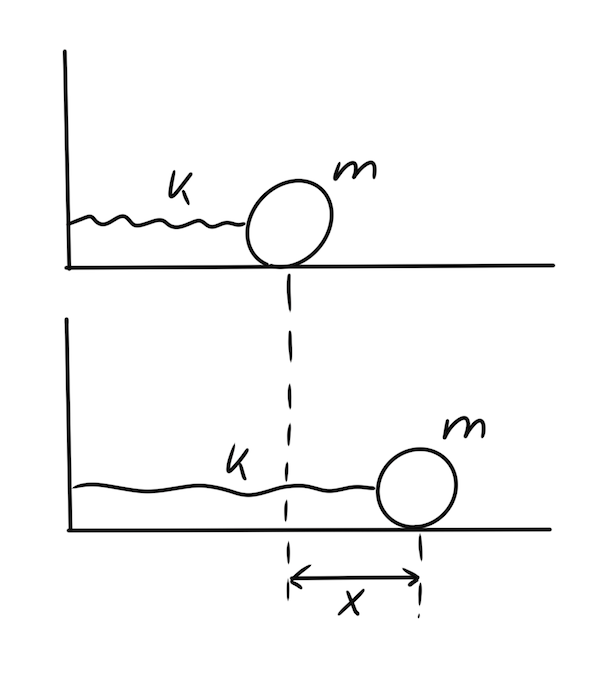
\includegraphics[width=0.3\textwidth]{/Users/vladbelousov/Desktop/Semestr_4-FP-NSU/ДфУ/Лекции_по_дням/image/17.png}
\end{center}

\[ T = \frac{m \dot{x } ^2 }{2} \quad  U = \frac{k x ^2 }{2}  \] 

\[ S = \int_{t_0 }^{t_1} \left( \frac{m \dot{x } ^2 }{2} -  \frac{k x ^2 }{2}\right)  dt \] 

Уравнение Эйлера (уравнение Лагранжа): \( \displaystyle  \frac{\partial L }{ \partial x  } - \frac{d}{dt} \frac{\partial L }{ \partial \dot{x}  } = 0  \) 

\[ - kx - \frac{d}{dt } ( m \dot{x } ) = 0  \Rightarrow m \ddot{x} + kx = 0  \] 

Понижение порядка: \( \displaystyle  L - \dot{x } \frac{\partial K }{\partial  \dot{x} } = C  \) 

\[ \frac{m \dot{x }  ^2 }{2 } - \frac{k x ^2 }{2 } - \dot{x } m \dot{x } = c \Rightarrow -\frac{m \dot{ x } ^2 }{2 } - \frac{k x ^2  }{2}  =c   \] 

\section{Изопериметрическая задача }

Найти кривую заданной длины, ограничивающую наибольшую площадь.

\[ \begin{aligned}
    S &\to  \max  \\ 
    l &= \mathrm{const}  
\end{aligned} \] 

\begin{center}
    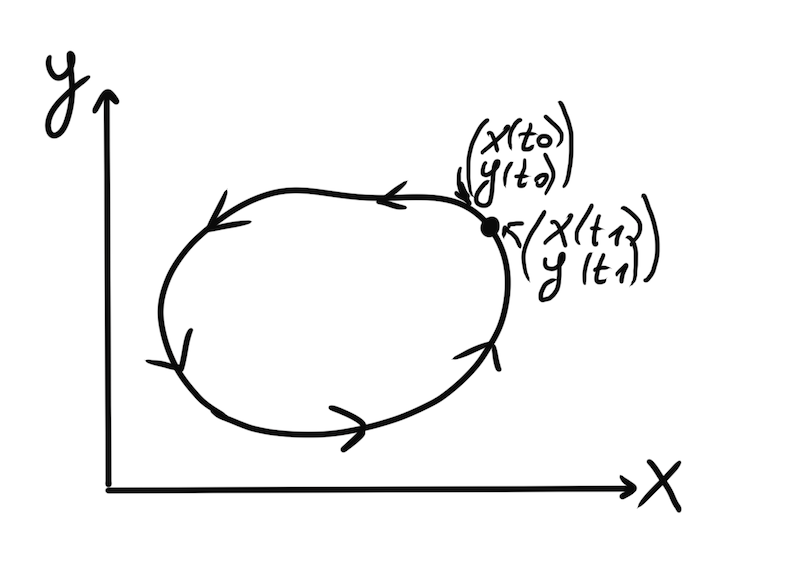
\includegraphics[width=0.5\textwidth]{/Users/vladbelousov/Desktop/Semestr_4-FP-NSU/ДфУ/Лекции_по_дням/image/18.png}
\end{center}

\[\begin{aligned}
    \begin{cases}
        x = x(t) \\ 
        y = y(t) \quad  t \in [ t_0 ,t_1]
        \end{cases}
    \begin{aligned}
        x(t_0 )=x(t_1) \\ 
        y(t_0 )=y(t_1) \\  
    \end{aligned}
\end{aligned} \]

\[ S = \iint_D dx dy   \] 

\[ \int_{ \partial D} \left( P(x,y )dx +Q(x,y )dy  \right) =\iint _D \left( - \frac{\partial P }{ \partial  y } (x,y ) + \frac{\partial Q}{\partial x }(x,y)   \right) dx dy\] 

\[ S = \iint_D dx dy = \iint_D \left(\underbrace{ \frac{1}{2 }}_{- \frac{\partial  P}{\partial y} } + \underbrace{ \frac{1}{2 }}_{ \frac{\partial  Q}{\partial x} }       \right)dx dy = \int_{ \partial  D } \left(  - \frac{y}{2 } dx + \frac{x}{2 } dy \right)  =\frac{1}{2 } \int_{t_0 }^{t_1} (x(t )y ' (t )- x' (t )y (t))dt  \] 

\[ \begin{cases}
\frac{\partial P } {\partial y } = -\frac{1}{2 }  \quad   \\
\frac{\partial Q }{\partial x } = \frac{1}{2 } \quad  Q = \frac{x}{2}   
\end{cases} \] 

\[ l = \int_{t_0 }^{t_1} \sqrt{(x' (t ) ^2 + (y '(t ) )^2 } dt = \mathrm{const}   \] 

Задача из математического анализа : 

\[ \begin{cases}
f(x_1, \ldots, x_n ) \to  \mathrm{extz}   \quad \quad  \tilde{f } =f + \lambda_1 g_1 + ... + \lambda_m g_m \to  \mathrm{extz}   \\
g_1 (x_1, \ldots, x_n ) = 0 \\
\vdots \\
g_m (x_1, \ldots, x_n ) = 0
\end{cases} \] 

Задача вариационного исчисления: 

\[ I[y_1, \ldots, yn] = \int_{x_0 }^{x_1 } F(x,y_1, \ldots, y_n,y_1',..., y_n') dx \to  \mathrm{extz}   \] 

\[ \begin{cases}
y_1(x_0 ) = y_0 ^1 \quad  y_n(x_0 ) = y_0 ^n \\
y_1(x_1 ) = y_1 ^1 \quad  y_n(x_1 ) = y_1 ^n \\
\end{cases} \] 

\[ Y[y_1, \ldots, y_n ] = \int_{x_0 }^{x_1} G(x,y_1, \ldots, y_n,y_1',..., y_n')dx = \mathrm{const}    \] 

Необходимое условие локального экстремума:

Пусть \( \tilde{y_1 }(x ),..., \tilde{y_n}(x) \) доставляет локальный экстремум функционалу \( I[y_1, \ldots, y_n] \)  и не является экстремалью функционалу \( Y[y_1, \ldots, y_n] \), тогда \( \exists  \lambda \in  \mathbb{R} \), такие, что \( \tilde{y_1}(x),..., \tilde{y_n}(x) \) доставляют экстремум функционалу \( \tilde{I } = I = \lambda Y \) 

\textbf{Без доказательства}

Замечание. \( I + \lambda Y \to  \mathrm{extz}  \Leftarrow \begin{cases}
    Y   = \mathrm{const}  \\
    I\to  \mathrm{extz} 
    \end{cases}  \) 

\[ \lambda \left( \frac{1}{\lambda }I + Y   \right) \to  \mathrm{extz} \Leftrightarrow Y+ \frac{1}{\lambda } \to  \mathrm{extz}  \Leftarrow \begin{cases}
Y \to  \mathrm{extz}  \\
I = \mathrm{const}  
\end{cases} \] 

Двойственная  задача: 

\[ \begin{aligned}
\begin{cases}
S \to  \max  \\
l = \mathrm{const}
\end{cases}
\Leftrightarrow 
\begin{cases}
l \to  \min  \\
S = \mathrm{const}
\end{cases}
\end{aligned} \]

\section{Решение классической изопериметрической задачи}

\[ \tilde{I } = S + \lambda l = \int_{t_0 }^{t_1 } \underbrace{\left[ \frac{1}{2 } (x y ' - x' y )+ \lambda \sqrt{(x') ^2 + (y ' ) ^2 } \right]}_{F}dt \to  \mathrm{extz}  \] 

\[ \begin{aligned}
    \begin{cases}
        \displaystyle \frac{\partial F }{\partial x } - \frac{d}{dt } \frac{\partial  F }{\partial  x ' } = 0 \quad  \\ 
        \vspace{0.01 mm} \\
        \displaystyle \frac{\partial F }{\partial y } - \frac{d}{dt } \frac{\partial  F }{\partial  y ' } = 0 \quad 
    \end{cases}
    \begin{cases}
        \displaystyle  \frac{1}{2 } y ' - \frac{d}{dt } \left[ -\frac{1}{2 } y + \lambda \frac{x ' }{\sqrt{(x') ^2 + (y ' ) ^2 }}  \right] =0\\
        \displaystyle -\frac{1}{2 } x ' - \frac{d}{dt } \left[ \frac{1}{2 } x + \lambda \frac{x ' }{\sqrt{(y') ^2 + (y ' ) ^2 }}  \right] =0 
    \end{cases}
\end{aligned}
\] 

№ 39.  Понизить порядок не получится так же, как в простейшей задаче.

\[ \begin{aligned}
    \begin{cases}
        \displaystyle \frac{d}{dt } \left[ \frac{y}{2 } + \frac{y}{2 } - \lambda \frac{x' }{\sqrt{(y') ^2 + (y ' ) ^2 }}  \right] =0 \\
        \displaystyle -\frac{d}{dt } \left[ \frac{x}{2 } + \frac{x}{2 } + \lambda \frac{y' }{\sqrt{(x') ^2 + (y ' ) ^2 }}  \right] =0
    \end{cases} 
    \begin{cases}
    \displaystyle y - c_1 = \frac{\lambda x' }{\sqrt{(x') ^2 + (y ' ) ^2 }} \\
    \displaystyle x - c_2 = \frac{-\lambda y' }{\sqrt{(x') ^2 + (y ' ) ^2 }}
    \end{cases}
\end{aligned}\] 

\[ \displaystyle (y- c_1 ) ^2 + (x- c_2 ) ^2 = \lambda ^2 \left[ \frac{(x') ^2 }{(x') ^2 + (y ' ) ^2 } + \frac{(y') ^2 }{(x') ^2 + (y ' ) ^2 } \right]  \] 

\[ \displaystyle (y- c_1 ) ^2 + (x- c_2 ) ^2 = \lambda ^2 - \text{окружность}  \] 

%%-------------------------------%%

% Закрытие документа, если файл компилируется отдельно
\ifdefined\mainfile
    % Если это основной файл, не нужно заканчивать документ
\else
    \end{document}
\fi
% Условная компиляция для самостоятельной работы
\ifdefined\mainfile
    % Если это часть основного файла, не добавляем начало и конец документа
\else
    \documentclass[12pt, a4paper]{report}
    \usepackage{/Users/vladbelousov/Desktop/Semestr_4-FP-NSU/Настройка/library}
    \usepackage[utf8]{inputenc} % Подключение поддержки UTF-8
    \begin{document}
\fi

%%-------------------------------%%

\section{Вариационная задача на условный экстремум}

\[ \begin{cases}
    I [y_1, \ldots, y_n]  = \int_{t_0 }^{t_1 }F(t,y_1, \ldots, y_n, y_n ',..., y_n')dt \to  \mathrm{extz}\\
    y_i (t_0 ) = y_{i_0}, \quad y_i (t_1 ) = y_{i_1} , \text{ }  i =1, \ldots, n\\
    G(t,y1, \ldots, y_n) = 0
\end{cases} \] 

Пример: Задача о геодезических на поверхности

\begin{center}
    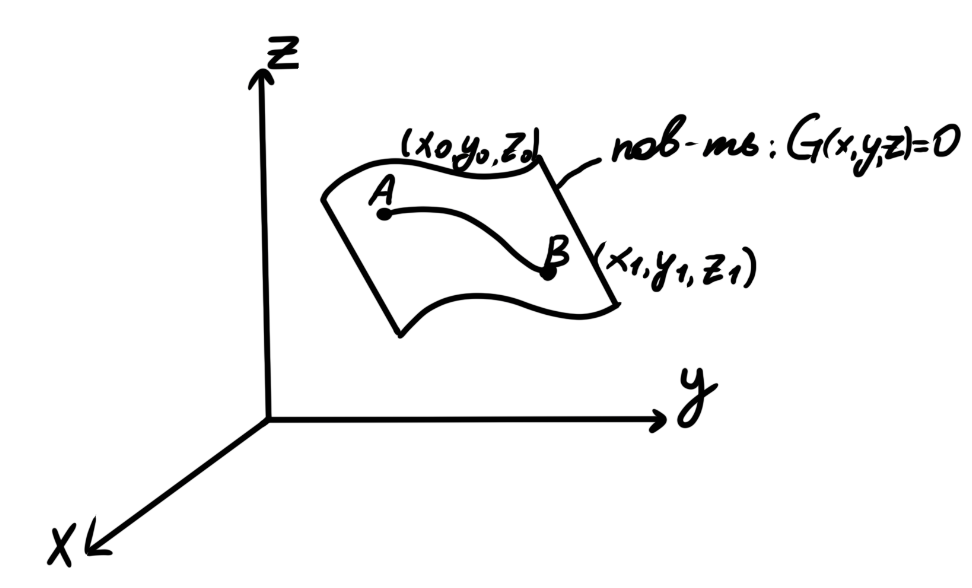
\includegraphics[width=0.5\textwidth]{/Users/vladbelousov/Desktop/Semestr_4-FP-NSU/ДфУ/Лекции_по_дням/image/19.png}
\end{center}

Найти кривую, соединяющую точки A и B, лежащие на поверхности, имеющую наименьшую длину. 

\[ \begin{cases}
x = x(t ) \\
y = y(t ) \quad  \text{уравнение кривой в параметрическом виде } ,\text{ }  t \in [t_0 , t_1]\\
z = z(t )
\end{cases} \] 

\[ I [x,y,z]  = \int_{t_0}^{t_1} \sqrt{(x' (t )) ^2 + (y' (t )) ^2 + (z' (t )) ^2 }dt \] 

\[\begin{cases}
x(t_0 ) = x_0 ,\quad x(t_1 ) = x_1 \\
y(t_0 ) = y_0 ,\quad y(t_1 ) = y_1 \\
z(t_0 ) = z_0 ,\quad z(t_1 ) = z_1
\end{cases} \] 

\textbf{Необходимое условие локального экстремума}:

Пусть \( \tilde{y_1 }, ..., \tilde{y }_n  \)  доставляют локальному экстремум для задачи (1). Тогда \( \exists    \lambda(t)   \) такая, что функции \( \tilde{y_1 }, ..., \tilde{y }_n  \) являются экстремалями вспомогательного функционала. 

\[ \tilde{I } [y_1, \ldots, y_n ] = \int_{t_0}^{t_1} (F + \lambda G(t))dt  \] 

\textbf{Без доказательства.} 

\section{Решение задачи о геодезических на сфере}

\begin{center}
    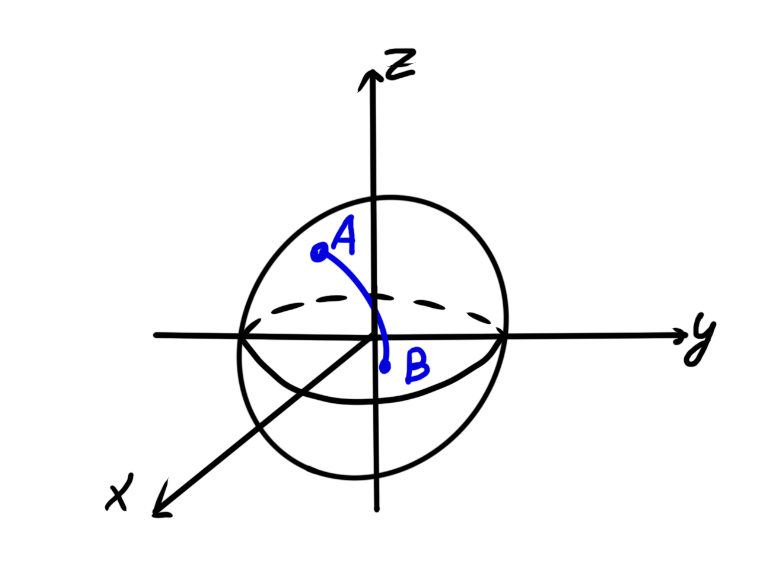
\includegraphics[width=0.4\textwidth]{/Users/vladbelousov/Desktop/Semestr_4-FP-NSU/ДфУ/Лекции_по_дням/image/20.png}
\end{center}

\[ x ^2  +y ^2 + z ^2 = R ^2  \] 

\[ I [x,y,z] = \int_{t_0}^{t_1} \sqrt{(x' (t )) ^2 + (y' (t )) ^2 + (z' (t )) ^2 }dt \] 

\[ \tilde{I } [x,y ,z ] = \int _{t_0}^{t_1}  \underbrace{\left(  \underbrace{\sqrt{(x' (t )) ^2 + (y' (t )) ^2 + (z' (t )) ^2 }}_{F}  + \lambda(t)(x ^2  +y ^2 + z ^2 - R ^2 ) \right)}_{\tilde{F}}  dt  \] 

\[\begin{cases}
    \displaystyle 2 x \lambda (t ) = \frac{d}{dt } \left( \frac{x' }{F}  \right) \quad (1)   \\
    \displaystyle 2 y \lambda (t ) = \frac{d}{dt } \left( \frac{y' }{F}  \right)  \quad (2)\\
    \displaystyle 2 z \lambda (t ) = \frac{d}{dt } \left( \frac{z' }{F}  \right) \quad (3)
\end{cases} \] 

\[ \begin{cases}
    \displaystyle (1) \cdot y + (2) \cdot (-x):\quad  y \frac{d}{dt } \left( \frac{x' }{F} \right) -x \frac{d}{dt } \left( \frac{y' }{F} \right) = 0 \\
    \displaystyle (2) \cdot z + (3 ) \cdot (- y) :\quad z \frac{d}{dt } \left( \frac{y' }{F} \right) -y \frac{d}{dt } \left( \frac{z' }{F} \right) = 0 \\
    \displaystyle (3) \cdot (-x) + (1) \cdot  z : \quad z \frac{d}{dt } \left( \frac{x' }{F} \right) -x \frac{d}{dt } \left( \frac{z' }{F} \right) = 0 
\end{cases} \] 

\[ \frac{d}{dt } \left( y \frac{x ' }{F }  - x \frac{y '}{F}  \right) = \cancelto{0}{y ' \frac{x ' }{F }} + y \frac{d}{dt } \left( \frac{x' }{F}  \right) \cancelto{0}{- x ' \frac{y '}{F}} - x \frac{d}{dt } \left( \frac{y' }{F}  \right) \] 

\[
\begin{aligned}
    \begin{cases}
        \displaystyle \frac{d}{dt } \left( y \frac{x' }{F } - x \frac{y ' }{F}  \right) = 0 \\
        \displaystyle \frac{d}{dt } \left( z \frac{y' }{F } - y \frac{z' }{F}  \right) = 0 \\
        \displaystyle \frac{d}{dt } \left( z \frac{x' }{F } - x \frac{z ' }{F}  \right) = 0 
    \end{cases} 
    \begin{cases}
        \displaystyle \frac{y x' - x y ' }{F } = c_1  \quad (1)\\
        \displaystyle \frac{z y' - y z ' }{F } = c_2  \quad (2)\\ 
        \displaystyle \frac{z x' - x z ' }{F } = c_3 \quad (3)
    \end{cases}
\end{aligned}\] 



\[ (1 )  \cdot z + (2)\cdot x + (3 ) \cdot (-y) : \]

\[ \frac{1}{F} \left[ z(y x' - x y ' ) + x (z y' - y z ' ) - y(z x' - x z ' ) \right] = c_1 z + c_2 x -  c_3 y  \] 

\[ \begin{cases}
    c_1 z + c_2 x -  c_3 y =  0 - \text{плоскость проходящая через (0,0,0)} \\
    x ^2 + y ^2 + z ^2 = R ^2 
\end{cases}  \] 

\begin{center}
    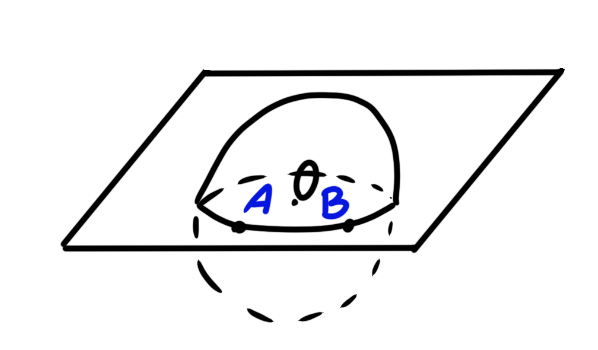
\includegraphics[width=0.3\textwidth]{/Users/vladbelousov/Desktop/Semestr_4-FP-NSU/ДфУ/Лекции_по_дням/image/21.png}
\end{center}

Геодезическая на сфере - дуга на большой окружности.

\chapter{Система малых колебаний}

\section{Линейные однородные системы малых колебаний}

\[ M \vec{x''}  + K \vec{x}  = 0  \quad  (1) \] 

\[ \vec{x }  =\vec{x } (t) = \begin{pmatrix}
x_1( t)\\
\vdots\\
x_n (t)
\end{pmatrix} \quad  M =\begin{pmatrix}
m_{11} & ... & m_{1n}\\
\vdots &  & \vdots\\
m_{n_1} & ... & m_{nn} 
\end{pmatrix} \quad K=\begin{pmatrix}
    k_{11} & ... & k_{1n}\\
    \vdots &  & \vdots\\
    k_{n_1} & ... & k_{nn} 
\end{pmatrix}  \]

Пример: \( n =1 \Rightarrow m x'' + kx = 0 , \text{ } m >0 , \text{ } k > 0 \) 

\begin{center}
    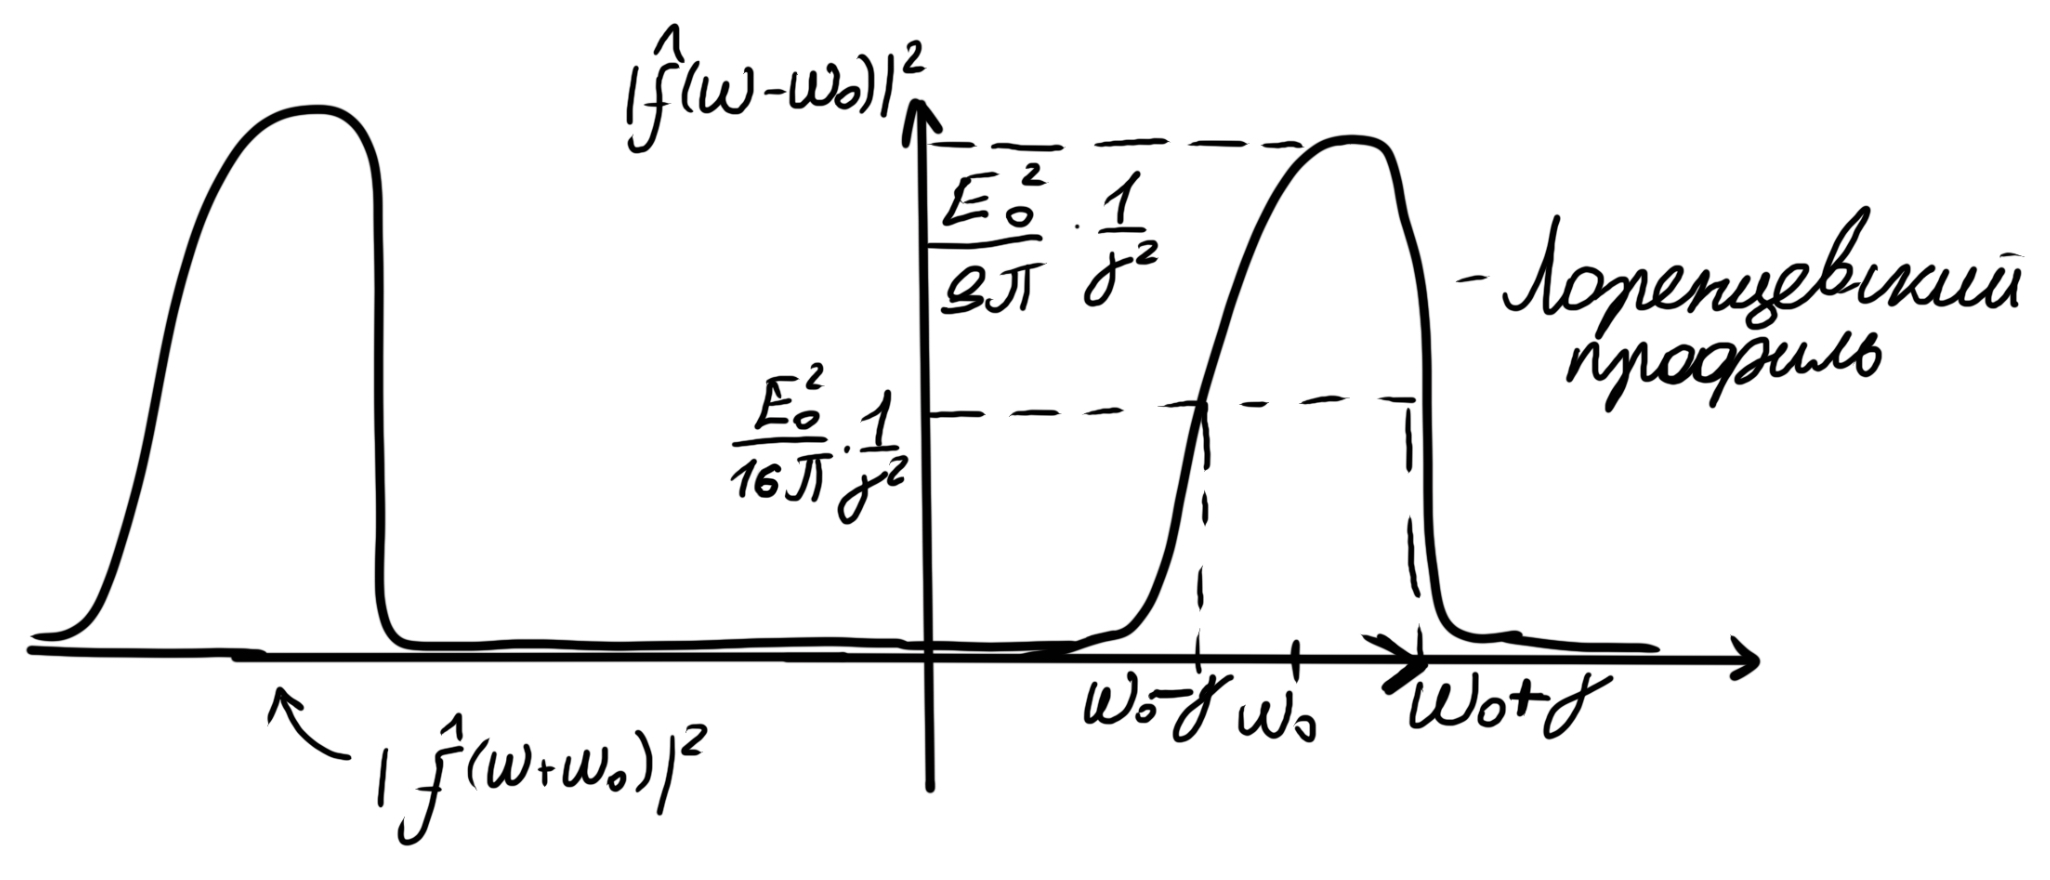
\includegraphics[width=0.3\textwidth]{/Users/vladbelousov/Desktop/Semestr_4-FP-NSU/ДфУ/Лекции_по_дням/image/22.png}
\end{center}

\[ M -\text{ матрица масс} , \quad  K -\text{ матрица жесткостей } \] 

1) \( M = M^{\top} , \text{ }  K = K^{\top}   \text{ } (m_{ij}= m_{j i} ,\text{ } k_{ij} = k_{j i}   ) \) 

2) M > 0  (матрица положительна определена), \( K \geq 0 \) 

\begin{definition}
    Матрица \( M = M^{\top} \) называется положительно определенной, если \( \forall \vec{v } \in  \mathbb{R} ^{n } , \vec{v } \neq 0  \) выполняется \( (M\vec{v} , \vec{v} ) >0 \).  
\end{definition}

\textbf{Критерий Сильвестра: } \( M = M^{\top} > 0 \Leftrightarrow  \text{все главные миноры} > 0. \)

\textbf{1-ый способ:} Сведение к системе 1-го порядка. 

\[ \begin{aligned}
    \begin{cases}
        \vec{y_1 } = \vec{x } \\
        \vec{y_2 } = \vec{x '} 
    \end{cases}
    \begin{cases}
        \vec{y_1 '} = \vec{y_2} \\
        \vec{y_2  '} = \vec{x ''} = -M ^{-1} K \vec{x }  = - M ^{-1} K \vec{y_1}   
    \end{cases}
\end{aligned} \] 

\[ \frac{d}{dt} \begin{pmatrix}
\vec{y_1} \\
\vec{y_2} \\
\end{pmatrix} = \underbrace{\overbrace{\begin{pmatrix}
    0 &  & E\\
     &  & \\
    -M^{-1}K  &  & 0
    \end{pmatrix}}^{A}}_{n \times n}  \begin{pmatrix}
\vec{y_1} \\
\vec{y_2} \\
\end{pmatrix}   \] 





\[ \begin{pmatrix}
    \vec{y_1} \\
    \vec{y_2} \\
\end{pmatrix} =\underbrace{e^{t A }}_{(2n \times  2n)} \underbrace{\vec{c}}_{(2n \times  1)}  = \begin{pmatrix}
\Phi_{11}(t) & \Phi_{12}(t)\\
\Phi_{12}(t) & \Phi_{22}(t)
\end{pmatrix} \begin{pmatrix}
\vec{c_1} \\
\vec{c_2} 
\end{pmatrix}  \]

\[ \vec{x} (t ) = \vec{y_1 } (t ) = F_{11} (t ) \vec{c_1 }  + F_{12} (t ) \vec{c_2 } \quad  (\text{2n констант} )    \] 

\begin{lemma}
    Если \( M = M^{\top} > 0  \), то \( \exists  M^{-1}  \)  
\end{lemma}

\begin{proof}
    \[  \] 
    Пусть не существует \( M^{-1} \Rightarrow \kern-30pt\underbrace{\mathrm{det } M = 0}_{\displaystyle \underset{ \displaystyle \det (M - 0 E) = 0}{\Rightarrow \lambda = 0 - \text{собств.знач.} }}\kern-30pt \Rightarrow \exists  \vec{v } \neq 0 : M \vec{v } = 0  \) 

    \[ (M\vec{v } , \vec{v }     ) = (0, \vec{v } ) = 0 - \text{  противоречие}  \] 
\end{proof}


\begin{proposition}[из алгебры]
    Пусть \( A = A^{\top} \Rightarrow  \)  все собственные числа \( \lambda_j \in  \mathbb{R}.  \) 

    Пусть  \( A = A^{\top} > 0 \Rightarrow  \) все собственные числа \( \lambda_j > 0.  \)
\end{proposition}

\begin{proposition}[из алгебры]
    Пусть \( A = A^{\top} \Rightarrow   \) в \( \mathbb{R} ^n  \)  существует базис из собственных векторов, то есть нет присоединенных 
\end{proposition}

\begin{proposition}[из алгебры]
    Пусть \( A = A^{\top} \Rightarrow A = U D U^{-1}  \), \( \begin{pmatrix}
    \lambda_1 &  & 0\\
    &\ddots  & \\
    0& & \lambda_n
    \end{pmatrix} \) 

\( U  \) - ортогональная  матрица, то есть \( U ^{-1} = U^{\top }   \)  
    
\end{proposition}

\textbf{2-ой способ:}

\begin{definition}
    Число \( \lambda     \)  называется собственным числом системы (1), если
    
    \( \det (K -\lambda M ) = 0 \) 
\end{definition}

\begin{definition}
    Вектор \( \vec{v }  \neq \vec{0}  \)  называется собственным вектором системы (1) (вектором нормальных колебаний), если \( (K -\lambda M ) \vec{v } = 0 \) 
\end{definition}

\begin{theorem}
    Существует n собственных чисел системы (1) и \( \lambda_{i } \geq 0 , \forall  i = 1,2,...,n \) 
\end{theorem}

\begin{proof}
\[  \]

1) \( \det (K -\lambda M )  = 0 \) 

\[ \det (M(M^{-1} K - \lambda E )) = 0 \] 

\[ \underbrace{\det M}_{ \neq 0} \det (M^{-1 } K - \lambda E ) = 0 \Rightarrow \text{ существует n собственных чисел}  \] 

2) \( \vec{v_j}  \)  - собственные вектора \( \Rightarrow K \vec{v_j} = \lambda_j M \vec{v_j} \text{ } | \cdot \vec{v_j}   \)  

\[ \underbrace{(K v_{j }  , v_j)}_{\geq 0}  = \lambda_j \underbrace{(M v_j ,v_j)}_{>0} \Rightarrow \lambda_j \geq 0  \] 
\end{proof}

\begin{theorem}
    В \( \mathbb{R} ^n \)  существует базис из собственных векторов системы (1).
\end{theorem}

\textbf{Доказательство будет позже.} 

\begin{theorem}
    Пусть  \( M = M^{\top} > 0 , K =K ^{\top} \geq 0 , \lambda_1, \ldots, \lambda_n \geq 0 \)  - собственные числа системы (1), \( \vec{v_1 },..., \vec{v_n}   \)  - собственные вектора системы (1), соответвующие числам \( \lambda_1, \ldots, \lambda_n \). Тогда все решения системы (1)  имеют вид: 

    \[ x(t) = \sum_{j=1} ^{n } q_j (t)\vec{v_j},   \] 

    , где \( q_j(t) \)  - решение дифференциального уравнения: \( q_j '' + \lambda_j q_j = 0 \) 
\end{theorem}

\begin{proof}
    \[  \] 
    По теореме 2 \( \vec{v_1},..., \vec{v_n }   \)  - базис в \( \mathbb{R} ^ n \). При фиксированном t \( x(t ) \in  \mathbb{R}^{n} \Rightarrow \vec{x } (t)  \)  раскладывается по базису: \( \vec{x } (t) = \sum_{j=1} ^{n } q_j (t)\vec{v_j}  \) 

    Подставляем \( x(t) \)  в систему (1): 

    \[ M \sum_{j =1}^n q_j '' (t ) \vec{v_j} + K \sum_{j =1}^n q_j (t ) \vec{v_j} = 0  \] 

    \[ \sum_{j=1}^ n \left( q_j '' (t ) M \vec{v_j } + q_j (t )\underbrace{ K \vec{v_j } }_{\lambda_j M \vec{v_j } } \right) =0\] 

    \[ \sum _{j=1}^ n \left( q_j '' (t ) M \vec{v_j } + \lambda_j q_j (t )M\vec{v_j }  \right) = 0 \text{ }  | \cdot  M^{-1}  \] 

    \[ \sum _{j=1}^ n \left( q_j '' (t  ) + \lambda_j q_j (t ) \right) \vec{v_j }= 0 , \text{ }  \forall  t \in  \mathbb{R}   \] 

    \[ \text{Т.к } \vec{v_1 },..., \vec{v_n} \text{ линейно независимы, то }  q_j '' (t ) + \lambda_j q_j (t) =0    \] 


\end{proof}

\begin{center}
    \textbf{Замечание.} \( q_j ''(t ) + \lambda_j q_j (t) = 0 \) 
    1) \( \lambda_j = 0 \Rightarrow q_j (t ) = c_1 t + c_2  \) 

    2) \( \lambda_j > 0 \Rightarrow q_j (t )  = c_1 \cos (\sqrt{\lambda_j} t) + c_2 \sin (\sqrt{\lambda_j} t) \)
\end{center}

\begin{definition}
    \( \omega_1 = \sqrt{\lambda_1},..., \omega_n = \sqrt{\lambda_n} \) называется собственными частотами колебаний системы (1).
\end{definition}

%%-------------------------------%%

% Закрытие документа, если файл компилируется отдельно
\ifdefined\mainfile
    % Если это основной файл, не нужно заканчивать документ
\else
    \end{document}
\fi

\vfill
\begin{center}
    \textbf{Пролетарии всех стран, соединяйтесь!}
\end{center}
\vfil

\end{document}